\documentclass[11pt,a4paper,openany]{memoir}\usepackage[]{graphicx}\usepackage[]{color}
%% maxwidth is the original width if it is less than linewidth
%% otherwise use linewidth (to make sure the graphics do not exceed the margin)
\makeatletter
\def\maxwidth{ %
  \ifdim\Gin@nat@width>\linewidth
    \linewidth
  \else
    \Gin@nat@width
  \fi
}
\makeatother

\definecolor{fgcolor}{rgb}{0.345, 0.345, 0.345}
\newcommand{\hlnum}[1]{\textcolor[rgb]{0.686,0.059,0.569}{#1}}%
\newcommand{\hlstr}[1]{\textcolor[rgb]{0.192,0.494,0.8}{#1}}%
\newcommand{\hlcom}[1]{\textcolor[rgb]{0.678,0.584,0.686}{\textit{#1}}}%
\newcommand{\hlopt}[1]{\textcolor[rgb]{0,0,0}{#1}}%
\newcommand{\hlstd}[1]{\textcolor[rgb]{0.345,0.345,0.345}{#1}}%
\newcommand{\hlkwa}[1]{\textcolor[rgb]{0.161,0.373,0.58}{\textbf{#1}}}%
\newcommand{\hlkwb}[1]{\textcolor[rgb]{0.69,0.353,0.396}{#1}}%
\newcommand{\hlkwc}[1]{\textcolor[rgb]{0.333,0.667,0.333}{#1}}%
\newcommand{\hlkwd}[1]{\textcolor[rgb]{0.737,0.353,0.396}{\textbf{#1}}}%

\usepackage{framed}
\makeatletter
\newenvironment{kframe}{%
 \def\at@end@of@kframe{}%
 \ifinner\ifhmode%
  \def\at@end@of@kframe{\end{minipage}}%
  \begin{minipage}{\columnwidth}%
 \fi\fi%
 \def\FrameCommand##1{\hskip\@totalleftmargin \hskip-\fboxsep
 \colorbox{shadecolor}{##1}\hskip-\fboxsep
     % There is no \\@totalrightmargin, so:
     \hskip-\linewidth \hskip-\@totalleftmargin \hskip\columnwidth}%
 \MakeFramed {\advance\hsize-\width
   \@totalleftmargin\z@ \linewidth\hsize
   \@setminipage}}%
 {\par\unskip\endMakeFramed%
 \at@end@of@kframe}
\makeatother

\definecolor{shadecolor}{rgb}{.97, .97, .97}
\definecolor{messagecolor}{rgb}{0, 0, 0}
\definecolor{warningcolor}{rgb}{1, 0, 1}
\definecolor{errorcolor}{rgb}{1, 0, 0}
\newenvironment{knitrout}{}{} % an empty environment to be redefined in TeX

\usepackage{alltt}

\setsecnumdepth{subsection}
\maxtocdepth{subsection}
\raggedbottom

\usepackage[hidelinks]{hyperref}
\usepackage[left=4cm, right=4cm]{geometry}
\usepackage{setspace}
\usepackage{graphicx}
\usepackage{subcaption}
    
\usepackage{calc,color}
\newif\ifNoChapNumber
\newcommand\Vlines{%
    \def\VL{\rule[-2cm]{1pt}{5cm}\hspace{1mm}\relax}
  \VL\VL\VL\VL\VL\VL\VL}
\makeatletter
\setlength\midchapskip{0pt}
\makechapterstyle{VZ43}{
  \renewcommand\chapternamenum{}
  \renewcommand\printchaptername{}
  \renewcommand\printchapternum{}
\renewcommand\chapnumfont{\Huge\bfseries\centering}
  \renewcommand\chaptitlefont{\Huge\bfseries\raggedright}
  \renewcommand\printchaptertitle[1]{%
    \Vlines\hspace*{-2em}%
    \begin{tabular}{@{}p{1cm} p{\textwidth-3cm}}%
      \ifNoChapNumber\relax\else%
      \colorbox{black}{\color{white}%
        \makebox[.8cm]{\chapnumfont\strut \thechapter}}
      \fi
      & \chaptitlefont ##1
    \end{tabular}
    \NoChapNumberfalse
}
  \renewcommand\printchapternonum{\NoChapNumbertrue}
}
\makeatother
\chapterstyle{VZ43}

\usepackage{polyglossia}
    \setmainlanguage{english}

\usepackage{fontspec}
    \setmainfont{FreeSerif}
    \frenchspacing
    \OnehalfSpacing
\usepackage{metalogo}

\usepackage{ctable,multirow,multicol,paralist,supertabular}

\usepackage{natbib}

\usepackage{gb4e}

\usepackage{mycleveref}


\title{Vowel duration and aspiration effects in Icelandic}
\author{Stefano Coretta}

\graphicspath{{./img/}}

\pagestyle{ruled}

%%%%%%%%%%%%%%%%
%%% DOCUMENT %%%
%%%%%%%%%%%%%%%%
\IfFileExists{upquote.sty}{\usepackage{upquote}}{}
\begin{document}









\frontmatter

\begin{titlingpage}
\maketitle
\end{titlingpage}

\tableofcontents*





\mainmatter


\chapter{Introduction}
\label{c:introduction}

This study deals with the relationship between the presence \textit{vs.} the absence of aspiration in a post-vocalic consonant and the duration of the vowel preceding that consonant.
\citet{maddieson1976,maddieson1976a} found that, in Hindi and a few other Indic languages, vowels followed by aspirated consonants (like in the word \textit{sāt} ``seven'') are longer than vowel followed by non aspirated consonants (like in \textit{sāth} ``companionship'').
This phenomenon has been subsequently called the ``aspiration effect'' by \citet{durvasula2012}, who further confirmed that the duration of vowel was related to aspiration.
Even if the effect has been shown to exist, no explanation has been given for it.
Moreover, these studies only dealt with post-aspiration.
To fully understand the phenomenon is necessary to extend the enquiry to pre-aspiration.

Such step has been taken in conducting this research.
Icelandic has been chosen as the language under study since its consonantal system can be interpreted as thoroughly based on aspiration contrasts.
In particular, aspiration in Icelandic involves both stops and sonorants consonants.
In certain contexts, non-aspirated geminate stops (/CC/) contrast with pre-aspirated stops (/ʰC/).
Similarly, voiced sonorants followed by a stop (/NC/) can contrast in the same contexts with voiceless sonorants followed by a stop (/N̥C/).
Since voiceless sonorants can be classed together with pre-aspirated stops, it is possible to explore the effect the presence of aspiration has on the duration of the preceding vowel.
The Icelandic phonological system thus constitutes an ideal locus of enquiry on the effects of aspiration on vowel duration in a more systematic way and in novel contexts than previously possible.

The studies on aspiration and vowel duration cited above showed that syllable-final \textit{post}-aspirated stops lengthened the preceding vowel.
These results are compatible with two opposite predictions with regard to \textit{pre}-aspirated stops.
In the simplest case, aspiration should consistently lengthen the vowel preceding the relevant consonant, independently of whether it is timed before or after the stop closure.
In a case where aspiration behaves symmetrically in relation to its timing, pre-aspiration should show a pattern opposite to that of post-aspiration, where the vowel preceding the pre-aspirated stop should be shorter.
If the second case is true, it could be asserted that the aspiration effect arises from the pattern of timing of the laryngeal spreading gesture in relation to the oral gestures.
I call this view the ``timing hypothesis,'' which will be the focus of this study.

\section{Research design}

This research has been designed so as to answer two questions: (1) does Icelandic show the aspiration effect? and (2) is the aspiration effect caused by the relative timing of laryngeal gestures in relation to oral gestures?
To access the existence of the aspiration effect in Icelandic, I collected data from native speakers.
They were recorded while reading a frame sentence which contained the target words.
The list of target words was selected so as to include aspirated and plain geminate stops and sonorants, both in word-final (in monosyllabic words) and word-medial position (in disyllabic words).
To test the validity of the laryngeal timing hypothesis, I performed a statistical analysis to verify the following research hypothesis: vowels followed by aspirated consonants (pre-aspirated stops and voiceless sonorants) are shorter than vowels followed by non-aspirated consonants (plain stops and voiced sonorants).


\section{Significance of the research}




\section{Reproducibility}
The term ``reproducible research'' was first coined by Prof. Jon Claerbout at Stanford University, around 2000 \citep{fomel2009}.
The concept of reproducible research stems from the idea the the product of the scientific inquiry should not only consist in the dissemination of the research results in the form of an output document (like a journal paper, a dissertation or a book).
Instead, such outcome should also include the environment in which the analysis that gave the results was performed.
Such an environment consists of the data sets and of the computational operations (in the form of code) used in the analysis.
A research is said to be reproducible when other people than the original authors can reproduce step by step the analysis that was conducted on the same data collected for that research.
While the concept of reproducibility might at first sight be similar to that of replicability, a scientific discovery is replicated when ``independent investigators, methods, data, equipment, and protocols'' are used \citep{peng2009}.

One way to satisfy the reproducibility criterion is using literate programming.
In literate programming, the computer code used to generate the results of the research is embedded within the research document.
The idea of literate programming has been developed by Donald Knuth \citep{knuth1984} as a way of simplifying the documentation process of computer programs.
This solution has been subsequently applied to scientific research, as a means for ensuring reproducibility.
Reproducibility and literate programming are new in linguistics, but some scholars are encouraging descriptive linguists to make their grammatical descriptions reproducible.
%TODO cite here 2 maxwell and maybe a third?

An interesting case in the area of phonology has been made by \citet{maxwell2013} regarding a theoretical debate based on data from Yokuts [\textsc{glotto}: \texttt{yoku1256}].
As \citet{weigel2002} and \citet{blevins2004a} pointed out, more than two thirds of the Yokuts lexical forms used as an argument in favour of theoretical claims turned out to be a construction of the researcher based on descriptions of the language.
What is worse is that those constructed word forms were incorrect.
More than thirty years of debate has been founded on false data.
The moral of this story is that linguistics as a whole would benefit from the application of reproducibility.
According to this spirit, this dissertation has been written in \XeLaTeX{} and \texttt{knitr}, a package that enables literate programming support in R \citep{r-core-team2015}.
%TODO explain better: say that it's in xelatex and that the analysis was in r because with knitr you can combine the two
The source code of the dissertation can be found at [...].
The dataset is downloadable at [...].


\section{Dissertation structure}
The dissertation is thus organised.
\Cref{c:review} contains a review of the literature relevant for the present study.
I will first introduce some background terminology and concept of the phonetics of laryngeal activity, followed by an overview of the relation between presence \textit{vs.} absence of aspiration and vowel duration.
Then, I will provide a brief description of the phonological system of Icelandic with a focus on the laryngeal contrasts in stops and sonorants.
The chapter closes with the statement of the research hypothesis.
\Cref{c:methodology} deals with the methodology of the experiment.
I will first discuss about the participants recruited for this study, the materials and the procedure used in the experimental task.
I will then give particular attention to the annotation scheme that was applied to the data and to the criteria used to extract the measurements.
In \Cref{c:results} I will present the results of the statistical analysis run on the extracted measurements.
Separate sections will deal with the duration of the words, the Voice Onset to Release (VOR), the vowels, the stop closure, the glottal spread gesture and of the sonorants.
\Cref{c:discussion} examines the results on the light of the research hypothesis.
This chapter also deals with the linguistics aspects of the research, its limitations and challenges, and the possible future implementations of this study.
Finally, concludes the dissertation with a summary of this work.

%TODO say about conventions? especially glottocodes, maybe even just in note, \citet{hammarstrom2016}






\chapter{Literature review}
\label{c:review}
This chapter contains the literature review of this study.
In \Cref{s:phonation}, I briefly introduce some basic concepts and terminology related to laryngeal activity in speech production.
\Cref{s:aspiration} deals with the phenomenon known as ``aspiration effect,'' according to which vowels followed by aspirated consonants are longer than when they are followed by non-aspirated consonants.
In \Cref{s:icelandic}, I discuss the major aspects of the phonology of Icelandic, focussing in particular on the laryngeal contrasts and contexts in stops and sonorants.
Finally, in \Cref{s:hypothesis}, I describe the hypothesis of this study and the reasons behind it.

\section{Phonation types and states of the glottis}
\label{s:phonation}
The periodic noise characteristic of the human voice is produced in the larynx.
In particular, the vibration of the vocal folds generates oscillations of the air pressure which is translated as a percept of periodic noise, or voicing, by the auditory system.
Even silence during speech is due to a particular configuration of the glottis (the empty space between the two vocal folds).
The larynx, with the vocal folds, thus plays a major role in human communication.

\citet{halle2002} review which configurations the vocal folds can assume.
Such configurations are known as the states of the glottis.
The four principal states of the glottis are (1) spread glottis, (2) constricted glottis, (3) stiff vocal folds, (4) slack vocal folds.
A spread glottis corresponds to abducted vocal folds.
This state is the one naturally used during normal breathing.
If the vocal folds are adducted so as they tightly press against each other, the glottis assumes a constricted configuration.
Independently from the first two states, the vocal folds can be either stiff or slack.
When the vocal folds are stiff, the distance between the upper and the lower edges of the folds is greater.
In the case of slack vocal folds, such distance is smaller and there is no tension in the vocal folds.
The first two states of the glottis can combine with the other two to create several phonation types.

\citet{ladefoged1973} discusses the four main phonation types that are employed to create phonological contrast in the languages of the world.
These are voicelessness, modal voice, breathy voice and creaky voice \citep{halle2002}.
A voiceless sound is produced with a laryngeal configuration that prevents vibration of the vocal folds.
The vocal folds can either be stiffened so as to prevent them vibrating, or abducted just enough to not allow enough pressure to build up and set off the vibration.
Modal voicing, instead, is produced with slack vocal folds and/or with adducted vocal folds.
When the transglottal pressure is sufficiently weak, the pressure of the airflow coming from the lungs can set the vocal folds to vibrate and produce a periodic sound, which is voicing.
Such mechanism of generating voicing is not the only one.
If the vocal folds are abducted enough to allow more airflow, but not as much as to prevent voicing, breathy voicing is produced.
On the contrary, if the vocal folds are constricted, the rate of vocal folds vibration decreases and voicing is characterised by a creaky sound (hence the term creaky voice).

When glottal spread is combined with voiceleness in stop consonants, the result is what is commonly known as aspiration.
Aspiration is, acoustically speaking, aperiodic noise in the higher frequency range generated by the substantial amount of airflow coming from the lungs through the abducted glottis.
In aspirated stops, aspiration normally follows the stop release, even if in certain languages aspiration is timed before the occlusion is made.
In the first case we talk about post-aspirated stops, while in the second of pre-aspirated stops.


\section{The effect of aspiration on vowel duration}
\label{s:aspiration}

Vowel duration has been reported in the literature to correlate with the presence vs. absence of aspiration in the following consonant.
In particular, \citet{maddieson1976} and \citet{durvasula2012} found that vowels followed by aspirated consonants in Hindi are longer than vowels followed by non-aspirated consonants.
In the following paragraphs, I will briefly introduce the system of laryngeal oppositions of Hindi.
I will then review some of the findings concerning the aspiration effect and the major theories regarding the cause of this phenomenon.

The consonantal system of Hindi is based on a four-way opposition of laryngeal contrasts \citep{ohala1983}.
For each place of articulation, there is a voiceless unaspirated, a voiced unaspirated, a voiceless aspirated and (breathy) voiced aspirated stop: for example, [t], [d], [tʰ], [dʱ].
The voiceless aspirated stops (like [tʰ]) are similar to the aspirated stops of English: a relatively long VOT follows the release of the occlusion.
The voiced counterpart (like [dʱ]) is normally voiced throughout the closure and the aspiration is characterised by breathy voicing.
\citet{maddieson1976} found that vowels followed by voiced and voiceless aspirated stops (like in [kaːd] `embroider' and [kaːtʰ] `wood') were of equal length but longer than vowels followed by voiceless stops (like in [kaːt] `cut').
Moreover, vowels followed by voiced aspirated stops (like in [saːdʱ] `balance') were even longer than voiced and voiceless aspirated stops.
\Cref{t:hindi} shows the mean duration of vowels before the four alveolar stops as reported by \citet{maddieson1976} and \citet{lampp2004}.

%ADD in note that phonemic is different
%ADD that no sd was given
\ctable[caption = Mean duration of vowels in Hindi when followed by dental and velar stops.\tmark,
label = t:hindi
]{llll}{
\tnote{The value of the standard deviation was not reported in the studies, so it is not included here.}
}{
\FL
\multicolumn{2}{l}{\citet{maddieson1976}} & \multicolumn{2}{l}{\citet{lampp2004}} \ML
consonant & vowel duration (msec) & consonant & vowel duration (msec) \ML
t       & 160    & k  & 188 \NN 
d       & 184.5  & g  & 187 \NN
tʰ      & 184.75 & kʰ & 217 \NN
dʱ      & 196    & gʱ & 221 \LL
}

\citet{lampp2004} could not replicate the findings in \citet{maddieson1976}.
\citet{durvasula2012}, however, performed a more controlled task and found clear evidence that aspiration lengthens the preceding vowel.\footnote{Voicing also played a role in the lengthening of vowels, where vowels followed by voiced stops were longer than vowels followed by voiceless stops, independently from aspiration.
Voicing and aspiration interacted so that a vowel followed by a voiced aspirated consonant was roughly two times longer than a vowel followed by a non-aspirated voiceless stop.
On the relation between vowel duration and voicing, see the following paragraphs.}
They also noted that an increase in closure duration of the stop following the vowel correlated with an increase of duration of the vowel, when controlling for other factors like voicing and aspiration.
The positive correlation between vowel duration and closure duration found in this study is the opposite of what has been found by \citet{maddieson1976} and \citet{lampp2004}.
Aspirated consonants in Hindi have a shorter closure duration than non-aspirated consonants.
Since vowels followed by aspirated consonants are longer, it is logical to assume that the shorter closure duration allows for the vowel to be longer, and, vice versa, the longer closure duration of non-aspirated stops makes the preceding vowel shorter.
However, since after controlling for confounds the duration of the vowel is positively correlated with closure duration, such explanation is not compatible.

\citet{maddieson1976} and \citet{durvasula2012} do not provide an explanation for the effect of aspiration on vowel duration.
Instead, they review proposals from other studies that dealt with a homologous phenomenon, the voicing effect.
The voicing effect states that vowels followed by voiced consonants are longer than vowels followed by voiceless consonants \citep{house1953,chen1970,hussein1994,durvasula2012}.
The voicing effect has been found in several languages, including English, Swedish, French, Arabic and Hindi \citep[191]{soskuthy2013}.
However, the strength and consistency of such effect vary depending on the language and on different contexts within one language.
While English has been reported to have a strong and consistent voicing effect, other languages, like Spanish, show a weaker effect \citep{hussein1994}.
On the other hand, yet other languages, such as Italian, have been shown to have no voicing effect at all \citep{esposito2002}.\footnote{\citet{laeufer1992}, however, argues that the differences in the strength of the effect are due to discrepancies in the experimental design.
Since this is not directly relevant to the present study, I refer the reader to \citet{laeufer1992} and references therein.
} 

Several explanations for the voicing effect have been proposed in the literature.
\citet{soskuthy2013} listed them into two categories.
One school of thought ascribes the voicing effect to articulatory properties of the consonant following the vowel \citep{belasco1953,chen1970}.
For example, \citep{belasco1953} argues that the voicing effect depends on the articulatory force needed to produce voiceless consonants.
Since, according to him, articulatory force is kept constant, vowels before voiceless stops are shortened to compensate for the higher articulatory force needed to produce them.
A second line of reasoning, instead, relates it to auditory principles \citep{javkin1976,kluender1988}.
Since the transition between vowels and voiced stops is gradual and does not have a clear boundary as with vowels followed by voiceless stops, \citep{javkin1976} argues that the voiced portion of the consonant is perceived to be part of the previous vowel.
In fact, \citet{maddieson1976} and \citet{durvasula2012} argue that none of the suggested explanations is satisfactory.
The majority of the studies makes incorrect predictions for vowel length followed by aspirated consonants, as found in Hindi.
In contrast, a promising line of enquiry emerges from the proposal by \citet{chomsky1968}, who attribute the voicing effect to adjustments of the larynx when moving from a vowel to a consonant.
%TODO probably need to expand on this


\section{Icelandic}
\label{s:icelandic}
%TODO contexts of laryngeal contrast

\ctable[caption = Major consonantal allophones of Icelandic.,
label = t:consonants
]{lccccc}{
\tnote{Note that some of the segments in the table are debated in the literature as to whether they are phonemic or just allophones.}
}{
\FL
& \textbf{labial}  & \textbf{coronal} & \textbf{palatal} & \textbf{velar} & \textbf{glottal}   \ML
\textbf{stops}      & p pʰ    & t tʰ    & c cʰ  & k kʰ    & ʔ \NN
\textbf{fricatives} & f v     & θ ð     & ç ʝ   & x ɣ     & h \NN
\textbf{nasals}     & m m̥    & n n̥    & ɲ ɲ̥  & ŋ ŋ̥    &   \NN
\textbf{laterals}   &         & l l̥    &       &         &   \NN
\textbf{trills}     &         & r r̥    &       &         &  \LL
}

Icelandic [\textsc{glotto}: \texttt{icel1247}] is spoken by the inhabitants of the Republic of Iceland (about 320,000 according to \citealt{arnason2011}), of which it constitutes the national language.
Icelandic is a Germanic language and, together with Faroese [\textsc{glotto}: \texttt{faro1244}], constitutes the Insular branch of the North Germanic group.
Among the Nordic languages, Icelandic and Faroese are the most conservative \citep{harbert2006,konig2013}.
%TODO say more about this

The modern phonological inventory of Icelandic has been subject to different analyses and it is still a matter of controversy \citep{thraisson1978,jessen1998,arnason2011}.
\Cref{t:consonants} reports the major consonantal allophones of Icelandic, as normally described in the literature \citep[98]{arnason2011}.
They do not necessarily represent the phonemic consonants of Icelandic and are rather surface segments.\footnote{
On the quarrel about the phonemic status of pre-aspiration and voiceless sonorants, see \citet{thraisson1978,jessen1998,berg2001,hansson2003,bombien2006}.
}
The consonantal system of Icelandic includes stops, fricatives, nasals, laterals and trills.
The places of articulation encompass labial, coronal (alveolar), palatal, velar and glottal.
Stops and fricatives have members in each place, nasals are labial, coronal, palatal and velar, while laterals and trills are coronal.
For each combination of manner and place of articulation there are two segments, one voiceless and one (voiceless) aspirated or voiced depending on the manner.
%TODO add about geminates -.-

The vocalic phonemes of Icelandic are given in \Cref{t:vowels} \citep[60]{arnason2011}.
On the antero-posterior axis, two places of articulation are distinctive: front and back.
On the vertical axis, vowels can be high, high-mid, low-mid and low.
Vowels can be either unrounded or rounded, even if a true phonemic contrast is present only in front-mid vowels.
Icelandic has the following diphthongs: the /i/-diphthongs /ai/, /ɛi/, /œi/, and the /u/-diphthongs /ou/, /au/.
The vocalic system of this language does not exploit phonological length distinctively.
Instead, vowels (both monophthongs and diphthongs) are predictably long when followed by two or more consonants, while they are short if one or no consonant follows.
For example: \textit{bað} /pað/ `bath' [paːð], \textit{kinn} /cɪnn/ `cheek' [cɪnn], \textit{baka} /pakʰa/  `to bake' [paːkʰa] and \textit{bagga} /pakka/ `burden.\textsc{acc}' [pakka]; \textit{álnir} /aulnɪr/ `wealth' [aulnɪr̥] ‘wealth’, \textit{ál} /aul/ `eel.\textsc{acc}' [auːl̥], \textit{álar} /aular/ `eels' [auːlar̥].\footnote{The actual distribution of long and short vowels is, unsurprisingly, debated.
For a review on the theoretical interpretations of the lengthening rule, see \citet{booij1986,pind1999}, and \citet[160--173, 203--208]{arnason2011}.
}

%TODO maybe add diphthgons as well!
\ctable[caption = Vocalic phonemes of Icelandic (monophthongs).,
label = t:vowels
]{lcccc}{}{
\FL
& \multicolumn{2}{c}{\textbf{front}}    & \multicolumn{2}{c}{\textbf{back}}   \NN
& \textit{plain} & \textit{rounded} & \textit{plain} & \textit{rounded} \ML
\textbf{high}     & i &   & & u \NN
\textbf{high-mid} & ɪ & ʏ  & &  \NN
\textbf{low-mid}  & ɛ & œ  & & ɔ \NN
\textbf{low}      &   &   & a & \LL
}

\subsection{Laryngeal contrasts in stops}
%TODO add examples
As mentioned in \Cref{s:aspiration}, the contrastive system of Hindi consonants is built on the cross-cutting interaction between aspiration and voicing.
Icelandic, on the other hand, contrasts only voiceless unaspirated with voiceless aspirated stops.
Voicing is reported to be totally absent in Icelandic stops, and does not appear even as passive voicing in intervocalic position \citep{arnason2011}.
The actual phonetic realisation of the aspirated series though varies depending on the variety it is spoken and on the phonological context.
In the so called ``soft'' variety of Icelandic (spoken everywhere in the island with the exception of the northern part), which is also the most widespread, aspiration is neutralised word-medially and word-finally, so that only non-aspirated stops can be found in those contexts.
For example: 
In the ``hard'' variety, spoken in the northern area of the island, the same neutralisation pattern occurs, but the unmarked member in the neutralisation---the one that emerges phonetically---is the aspirated one.
In this variety, stops are aspirated in every context, but they contrast with non-aspirated stops at the beginning of a word.

Moreover, aspirated geminate stops, both word-medially and word-finally, are realised as pre-aspirated stops.
For example: .

\subsection{Laryngeal contrasts in sonorants}
The Lyon-Albuquerque Phonological Systems Database (LAPSyD) phonological data\-base \citep{Maddieson2012} states that 51 out of 586 languages of the world use laryngeal settings contrastively in sonorants.
The contrastive use of laryngeal distinctions in sonorants can thus be considered cross-linguistically rare (only 8.7\% of languages in LAPSyD have this property).
Unsurprisingly, sonorants produced with modal voicing are the most common type.
If more than one phonation type is used in sonorants to accomplish phonological contrasts, at least one of those is always modal voicing.
Icelandic is among those rare languages that show voicing contrasts in sonorants and it has voiced and voiceless nasals, laterals and trills.
In the following paragraphs I will show how the voiceless sonorants of Icelandic can be though of as aspirated consonants.
This interpretation makes it possible to group both the aspirated consonants and the voiceless sonorants under a single category ``aspirated.''
Such move will prove to be useful for the development of the hypothesis in the present study.

\citet{ladefoged1996} discuss the possible combinations of phonation types and oral gestures in nasal consonants.
Apart from modal voicing, three other types of phonations are found among nasals in the languages of the world: breathy voice, creaky voice and voicelessness.
Breathy and creaky voice will not be dealt with here, since they are not immediately relevant for this study.
\citet{bhaskararao1991} state that voicelessness in nasals is implemented in two possible ways.
The type known as the ``Burmese type,'' which is also the most common, is constituted by an initial portion of voicelessness followed by a portion characterised by modal voicing (bilabial [N̥͡mV], and alveolar [N̥͡nV]).\footnote{Since place cues are not recoverable during the voiceless part of the nasal, the capital letter ⟨N⟩ is used to indicate placelessness.
This solution is used by \citet{silverman2012}.
}
In the second type of voiceless nasals, the segment is voiceless through out its duration.
However, when oral occlusion is released, the velum is still open, so that the nasal port is unobstructed.
Since the velum is open, air can freely escape through the nasal cavity.
The small burst produced by releasing the occlusion mimics the auditory features of an epenthetic stop \citep[84]{bhaskararao1991}.
Such configuration could be represented as [N̥ᵖV] for the bilabial nasal and [N̥ᵗV] for the alveolar one.

\citet[111]{ladefoged1996} say that the nasal airflow of the voiceless nasals of Burmese is very high.
Since air comes from the lungs and the oral cavity is closed by the tongue, the airflow rate is correlated with the amount of glottal width.
A high nasal airflow seems thus to suggest that voiceless nasals are produced with abducted vocal folds.
Due to this property, the researchers argue that voiceless nasals in general are perhaps better described as ``aspirated.''
\citet[82]{kehrein2002}, based on \citet{ladefoged1996}, interprets voiceless nasals as phonologically aspirated.

% They are reported to be usually longer in comparison to their voiced counterparts \citep[111]{ladefoged1996sounds}.

As with nasals, laterals and trills can use phonation types contrastively, included voicelessness.
Voiceless laterals can be realised as either approximants or fricatives \citet{ladefoged1996}.
These two way of implementing voiceleness in laterals can be distinguished according to a variety of acoustic parameters.
Given that in approximants the vocal tract is open while in fricatives it is more constricted, approximants are normally characterised by ``a lower amplitude of noise, a greater tendency to anticipate the voicing of a following vowel, and a concentration of energy lower in the spectrum than voiceless fricative laterals'' \citep[198]{ladefoged1996}.

Trills are made up by a sequence of quickly repeated closures produced in the oral cavity.
Voiced trills are characterised by the presence of voicing during the intervals between each closure.
In voiceless trills, instead, voicing is absent between the closures that constitute the trill \citep[236]{ladefoged1996}.
%For

\citet{helgason2002} notes how the phasing of the laryngeal gestures in pre-aspirated stops resembles the one in voiceless sonorants.
In both cases, the peak of glottal spread is achieved before the stop closure.
Moreover, the voice offset is simultaneous with stop closure in plain geminates and voiced sonorants, while it occurs before the stop closure in both pre-aspirated geminates and voiceless sonorants.
Such similarity in the relative timing of oral and laryngeal gestures strengthens the idea that pre-aspirated geminates and voiceless sonorants in Icelandic could be treated as members of a single class of aspirated or spread glottis consonants.

%TODO maybe expand on the following
\citet{bombien2006} reports that voiceless sonorants in Icelandic have the following acoustic properties: 
\begin{inparaenum}[(i)]
\item voiceless sonorants are longer in duration than their voiced counterparts;
\item they have greater H1-H2 (first and second harmonic) difference than the voiced ones (which indicates breathy phonation in the former);
\item they show greater zero crossing rate values (which indicates higher frication compared to the voiced sonorants).\footnote{Frication has been proved to create higher frequencies compared to non-fricated sounds and hence it involves higher rate of zero crossing \citep{weigelt1990}.}
\end{inparaenum}

\subsection{Phonotactics}

Relevant to this study is the way phonation types are exploited to create contrast in stop and sonorant consonants in Icelandic.
Even if the phonemic oppositions are ideally straightforward---non aspirated consonants contrast with non-aspirated ones---the actual phonotactic distribution of contrastive consonantal segments is quite complex.
There are restrictions on possible contrasts depending on the position within the word and the preceding or following segments. Except word-initially, both plain and aspirated stops can be geminated.
\Cref{t:contrasts} shows the distributions of contrasts in stops and sonorants in various contexts within the word.
The labial stops and the alveolar nasals are used as an exemplification, respectively, of the distribution of stops and sonorants.

\ctable[caption= Possible phonation and gemination contrasts in Icelandic ordered by context.,
label= t:contrasts
]{cccccccc}{}{
\FL
                                    & \#\_  & \multicolumn{2}{c}{V\_V} & V\_(l/n) & V\_C & \multicolumn{2}{c}{\_\#}  \ML
\multirow{3}{*}{\textit{stops}}     & p     & p  &    & p  &    & p &  \NN
                                    &       &    & pp &    &    &   & pp  \NN
                                    & pʰ    &    & ʰp & pʰ &    &   & ʰp \NN
\multirow{2}{*}{\textit{sonorants}} & n     & n  &    &    & n  & n̥ &   \NN
                                    & n̥     &    &    &    & n̥  &   &    \LL
}


\section{Research hypothesis}
\label{s:hypothesis}

The studes by \citet{maddieson1976} and \citet{durvasula2012} showed that syllable-final \textit{post}-aspirated stops lengthened the preceding vowel.
These results are compatible with two opposite predictions with regard to \textit{pre}-aspirated stops: either aspiration consistently appears to lengthen the preceding vowel, independently of the relative timing with the stop closure; or pre-aspiration should show a pattern symmetric to that of post-aspiration, where pre-aspirated stops should be preceded by shorter vowels.
%ADD about sonorants!

The hypothesis I propose in this study rests on the idea that the aspiration effect is the product of the relative alignment of the glottal spreading gesture and the oral gesture.
Depending on how the spreading of the glottis is timed in relation to the tongue gestures in the oral cavity, modal voicing can be maintained for a certain amount of time or it is terminated earlier.
An early timing of glottal spreading (like in pre-aspiration) would prevent voicing in the last portion of the preceding vocalic gesture, making the vowel shorter.
On the contrary, if the spreading gesture is timed later relative to the oral gesture (like in post-aspiration), the voicing in the preceding vowel can be sustained, leading to a longer vowel.
In a language like Hindi that contrasts non-aspirated with post-aspirated stops, a vowel followed by a post-aspirated stop would be relatively longer than a vowel followed by a non-aspirated stop since in the former case the spreading gesture that allows post-aspiration should allow more voicing.

In Icelandic, the contexts where a contrast involving aspiration can be found post-vocalically is with geminates stops, RC clusters (/l/ or /r/ + stop) and NC clusters (nasal + stop) in word-medial and final position.
As mentioned above, aspiration is realised as pre-aspiration in geminate stops and as (partial) voicelessness in sonorants.
If the timing interpretation of the aspiration effect is correct, vowels before pre-aspirated geminates and voiceless sonorants should be shorter than vowels before plain geminates and voiced sonorants.
Given that pre-aspirated stops and voiceless sonorants can be categorised under the umbrella term ``aspirated consonants'' (for the reasons above), these two separate statements can be merged into a single hypothesis:

\begin{exe}
\ex\label{h1} \textbf{Alternative hypothesis} (H\textsubscript{1}) \\
Vowels followed by aspirated consonants are shorter than vowels followed by unaspirated consonants.
\end{exe}

The corresponding null hypothesis is:

\begin{exe}
\ex\label{h0} \textbf{Null hypothesis} (H\textsubscript{0}) \\
Vowels followed by aspirated consonants are of the same duration as vowels followed by unaspirated consonants.
\end{exe}

%TODO section on prosodic approach and articulatory phonology?






\chapter{Methodology}
\label{c:methodology}
%TODO prosodic approach
In this chapter I will describe the methodology employed for this study.
\Cref{s:participants} contains information about the speakers that participated in the study.
In \Cref{s:materials}, I detail the materials used in the task, which is outlined in \Cref{s:procedure}.
\Cref{s:annotation} discusses the annotation scheme, and the criteria employed in the annotation.
Separate subsections deal with the labelling parameters for the detection of, respectively, word boundaries, voicing, glottal spread, nasality, laterality, rhoticity, and stop release.
\Cref{s:measurements} defines the measurements that I extracted from the annotated files and describes the procedure used for data normalisation.
Finally, \Cref{s:stats} briefly mentions the features of the statistical analysis applied to the measurements and the software I used to implement it.

\section{Participants}
\label{s:participants}

For this study, I recruited six Icelandic speakers who were living in York (UK) at the time the recordings were made.
The methodologies of this research have gained the approval of the Ethics Committee and the subjects received an information sheet and signed a consent form.
Recruitment was done through University channels, the Icelandic Embassy in London and the York Anglo Scandinavian Society.
All the participants were native speakers of Icelandic, above 18 years old and claimed to have normal hearing and speech abilities.
The informants received a compensation for their time in the form of Amazon vouchers or chocolates for the value of £5 pounds.

The information on each participant is given in \Cref{t:participants}.
The column labelled ``birthplace'' contains the city or town where the subjects were born; the eventual city or town in parenthesis is the place where they spent most of their life if different from their birthplace.
The last column, ``abroad'', states if the subjects spent more that 6 months outside Iceland.
The participant JR had to be excluded from the analysis since he misunderstood the task, while part of the participant SHG's task was lost due to a technical fault in the recording equipment.
All the speakers were from the Southern parts of Iceland so they are assumed to speak the ``soft'' variety of Icelandic.


\ctable[caption = Information on participants.,
label = t:participants,
]{cccclc}{}{
\FL
\textbf{id} & \textbf{sex}    & \textbf{age} & \textbf{birthplace} & \textbf{languages} & \textbf{abroad} \ML
TT & female & 24 & Reykjavik & English, Danish, German  & Yes \NN
BRS & female & 25 & Hofn      & Danish, English, Spanish & Yes \NN
BTE & female & 27 & Reykjavik & English, Danish          & Yes \NN
JJ & female & 46 & Reykjavik (Kopavogur) & English, Danish          & Yes \NN
SHG & male   & 25 & Selfoss   & English                  & No  \NN
JR & male   & 66 & Reykjavik (York)      & English                  & Yes \LL
}

\section{Materials}
\label{s:materials}
%TODO say that geminates or simply stops are equivalent in this thesis due to the phnotactics and the design; maybe use TT for stops only!
The material used in the task consisted of a list of Icelandic words (the ``target words'') with the following forms: (C)VCC (monosyllabic) and (C)VCCV (bisyllabic).
The list of target words is given in \Cref{t:wordlist}.
The target words were selected so as to control for as many of the following aspects as possible: phonation, manner and place of articulation of consonants following the target vowel; height and frontness of the target vowel; phonation, manner and place of articulation of consonants preceding the target vowel; and height and frontness of the eventual word-final vowel.
Control over these parameters was prioritised according to the order in which they were presented here.
Unfortunately, obtaining a well controlled word list proved to be extremely difficult and several compromises have been made.
%TODO CITE holes and humps papers!

The wordlist contained a total of 58 inflected Icelandic words (only real word forms were used).
These were a mixture of nouns (26), verbs (22), adjectives (8) and adverbs (2).
The 58 words were equally divided in monosyllabic (29) and bisyllabic (29) words.
Of the monosyllabic words, 20 ended with a geminate stop (9 plain geminates and 11 pre-aspirated geminates); 5 with an /NC/ cluster (2 voiced and 3 voiceless nasals); 2 with an /lC/ cluster (one voiced, one voiceless); one word ended with a geminate nasal.
Of the bisyllabic words, 14 had a word-medial geminate stop (8 plain and 6 pre-aspirated); 9 a /NC/ cluster (5 voiced and 4 voiceless); 4 an /lC/ cluster (2 voiced and 2 voiceless); and 2 had an /rC/ cluster (one voiced, one voiceless).

%TODO tokens! I talk about types but should talk about tokens as well

\vspace{5em}

\tablefirsthead{
    \hline
	word\hspace{2cm}    & IPA\hspace{2cm}          & pos\hspace{2cm} & gloss \hspace{2cm}  \\
	\hline}
\tablehead{
    \hline
    word\hspace{2cm}    & IPA\hspace{2cm}          & pos\hspace{2cm} & gloss \hspace{2cm}  \\
    \hline}
\tablecaption{List of target words.}
\label{t:wordlist}

\begin{supertabular}[t]{llll}
\multicolumn{4}{l}{stops}				   \\ \hline
kokk  & kʰoʰk  & noun      & cook          \\
gogg  & kokk   & noun      & beak          \\
dökk  & tœʰk   & adjective & dark          \\
dögg  & tœkk   & noun      & dew           \\
kopp  & kʰoʰp  & noun      & chamber pot   \\
kubb  & cʰʏpp  & noun      & block of wood \\
vítt  & viʰt   & adverb    & far and wide  \\
vídd  & vitt   & noun      & width         \\
þítt  & θiʰt   & verb      & thaw          \\
þíddi & θittɪ  & verb      & thaw          \\
fætt  & faiʰt  & verb      & feed          \\
fæddi & faittɪ & verb      & feed          \\
ýtt   & iʰt    & verb      & push          \\
ydd   & ɪtt    & verb      & sharpen       \\
ótt   & ouʰt   & noun      & point         \\
odd   & ott    & adverb    & fast          \\
sets  & sess   & noun      & sediment      \\
sett  & seʰt   & verb      & put           \\
feits & feiss  & adjective & fat           \\
feitt & feiʰt  & adjective & fat           \\
vots  & voss   & adjective & wet           \\
vott  & voʰt   & adjective & wet           \\
takka & tʰaʰka & noun      & key           \\
kagga & kʰakka & noun      & barrel        \\
detta & teʰta  & verb      & fall          \\
gedda & cetta  & noun      & pike          \\ \hline
\multicolumn{4}{l}{nasals}				   \\ \hline
kamp   & kʰam̥p  & noun      & moustache       \\
kamb   & kʰamp   & noun      & comb            \\
punt   & pʰʏn̥t  & noun      & decoration      \\
pund   & pʰʏnt   & noun      & pound           \\
kembt  & cʰem̥t  & verb      & comb            \\
kembdi & cʰemtɪ  & verb      & comb            \\
kampa  & kʰam̥pa & noun      & moustache       \\
kamba  & kʰampa  & noun      & comb            \\
kempa  & cʰem̥pa & noun      & hero            \\
kemba  & cʰempa  & verb      & comb            \\
punta  & pʰʏn̥ta & noun      & decoration      \\
punda  & pʰʏnta  & noun      & pound           \\
vanta  & van̥ta  & verb      & want            \\
vanda  & vanta   & verb      & do st carefully \\
fínn   & fitn̥   & adjective & smart           \\
kinn   & kʰɪnn   & noun      & cheek          \\ \hline
\multicolumn{4}{l}{laterals}				   \\ \hline
duld   & tʏlt     & adjective & complex  \\
dult   & tʏl̥t    & adjective & reticent \\
gelta  & cel̥ta   & verb      & bark     \\
gelda  & celta    & verb      & castrate \\
mjólka & mjoul̥ka & verb      & milk     \\
ólga   & oulka    & verb      & foam    \\ \hline
\multicolumn{4}{l}{trills}				   \\ \hline
orka   & or̥ka    & noun      & energy   \\
orga   & orka     & noun      & scream   \\ \hline
\end{supertabular}


\section{Procedure}
\label{s:procedure}
The target words were embedded in the frame sentence \textit{Segðu \_\_ aftur}, `Say \_\_ again.'
This sentence was chosen with the aid of one of the participants so as to control for naturalness, number of syllables and phonetic contexts preceding and following the target word, and phrase stress.
The decision to use a single frame sentence for all the test words was justified by the will of keeping the task as simple as possible.
The participants were asked to read aloud the sentences with the target words shown on a computer screen.
They were advised to speak as naturally as possible, while keeping the same volume and pace.
They did not familiarised themselves with the word list before starting the task.
The decision of not showing the words beforehand was made to reduce the speakers' control over their speech.

The task was presented through the software PyschoPy \citep{peirce2009}, on a Apple MacBook Pro.
Each sentences was shown three times consecutively and the order of appearance was randomised across subjects.
The reading task was self-paced; the participant read a sentence shown on the screen and moved to the next sentence when ready by pressing the space bar.
Four speakers were recorded in York in a meeting room at the travel agency they worked for, while one was recorded at the University of York.
One speaker did not agree at coming to the University Campus, so he was recorder in his living room, at his house in York.
The only subject who performed the task at the University of York was recorded in a sound-proof studio, using a Beyerdynamic OPUS 54 headset microphone (condenser, cardioid), plugged into a recording station.
The software used for the recording was Adobe Audition, running on a Windows computer.
The other speakers were recorded using the same headset microphone plugged into a Zoom H4n Handy Recorder.
The audio files were encoded using the \texttt{.wav} format at a sampling rate of 44 kHz (16-bit).
Even if the recording conditions differed between participants, the quality of the audio is comparable across files.

\section{Annotation}
\label{s:annotation}

\begin{figure}
\centering
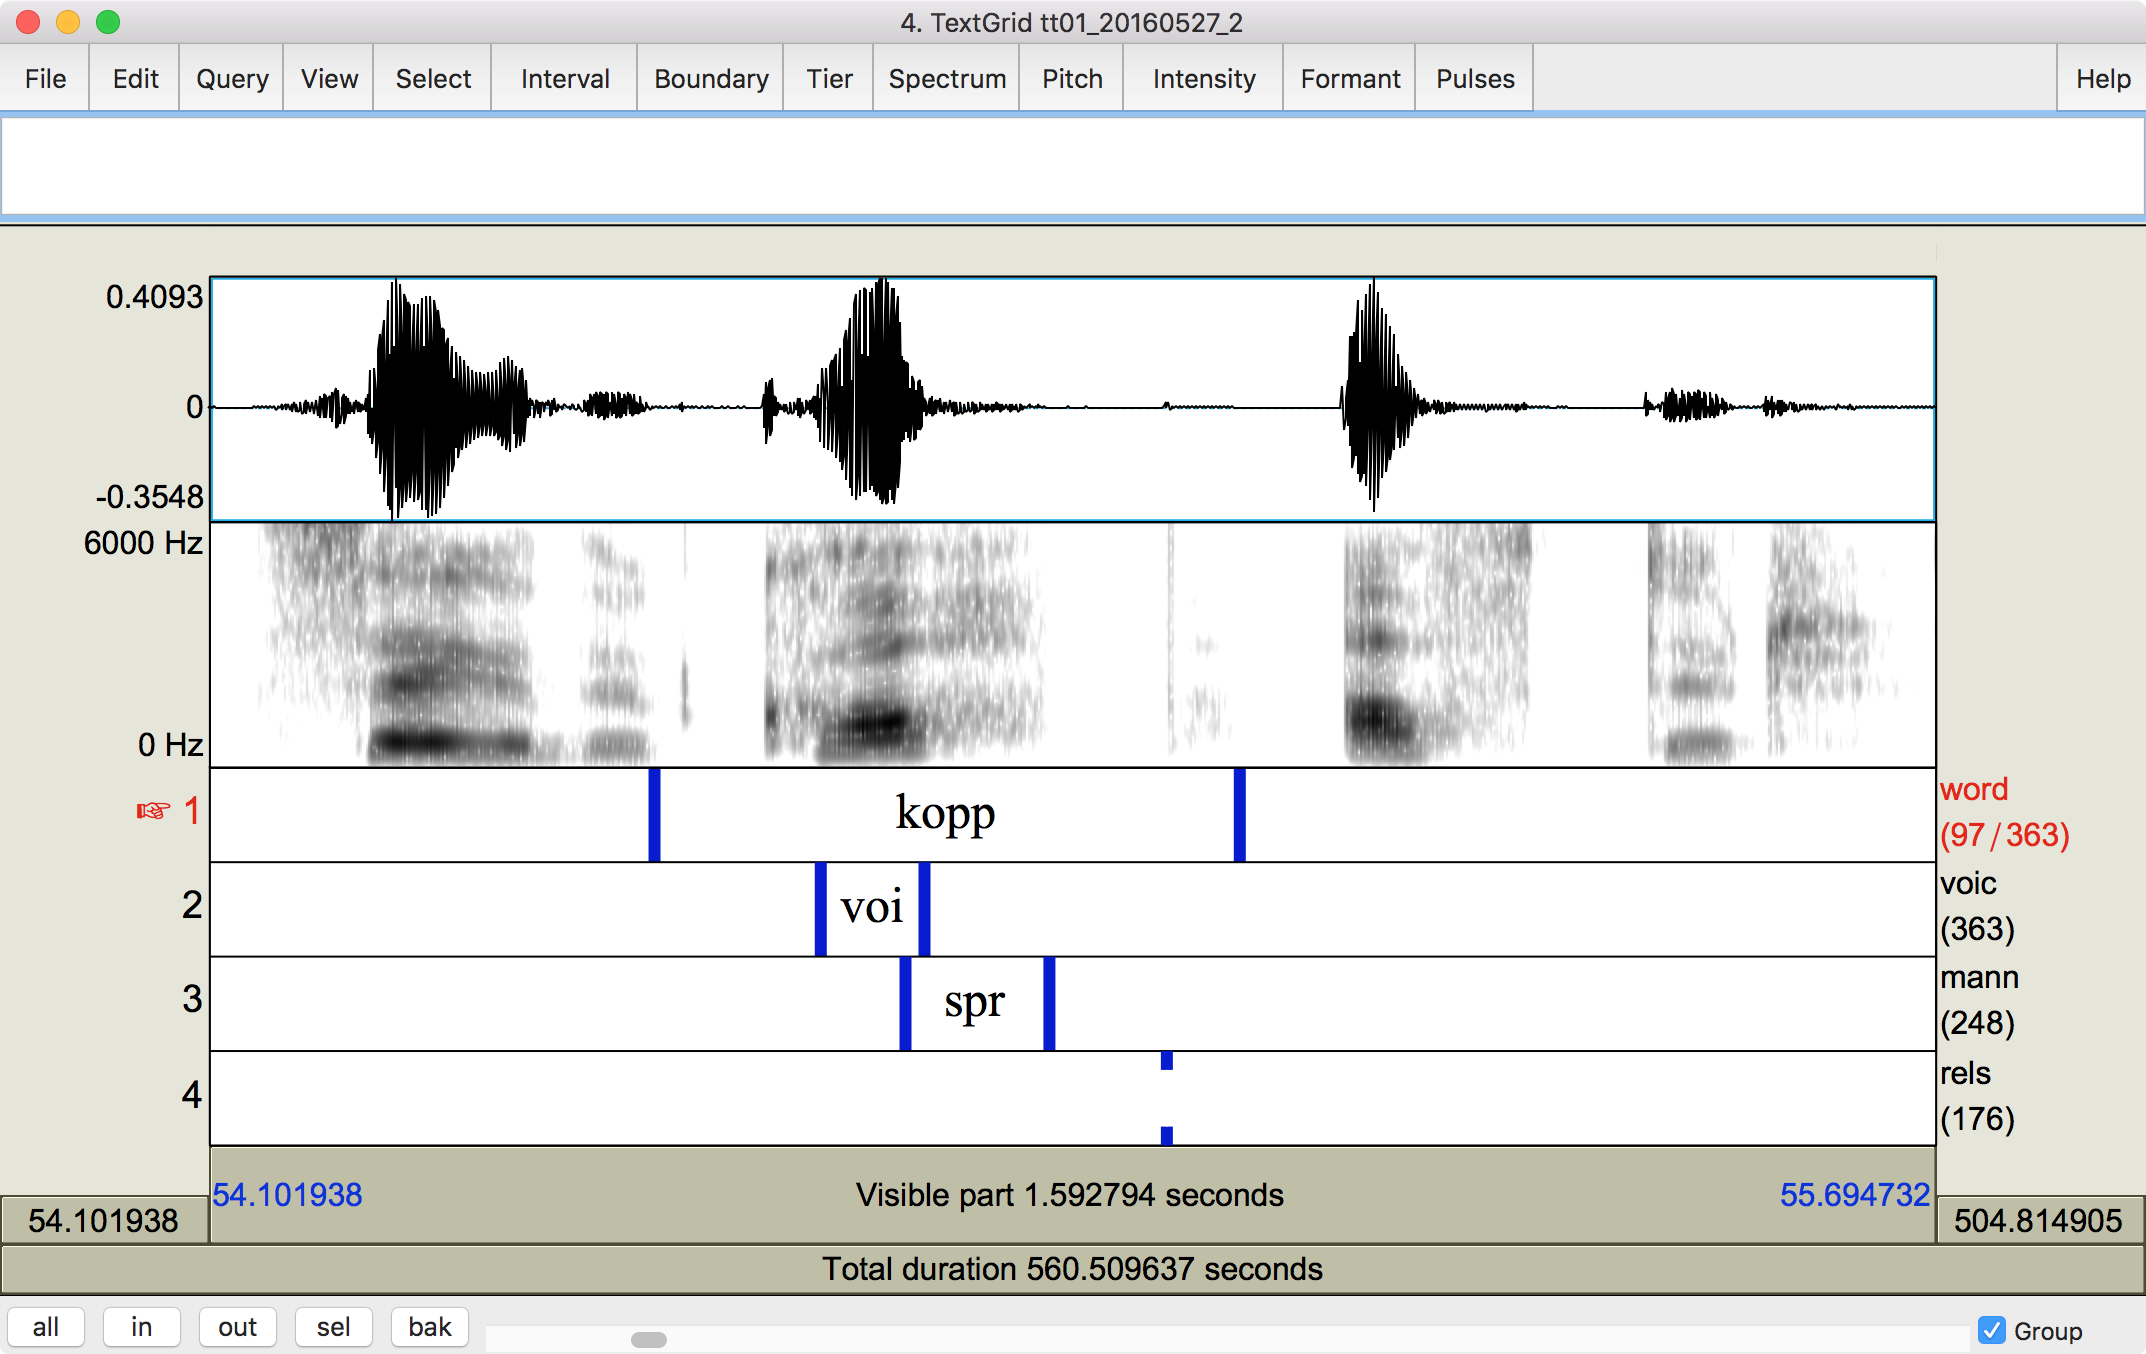
\includegraphics[width=\textwidth]{textgrid}
\caption{Example of the tier structure of the annotation files (PRAAT TextGrids). Tiers: 1. \texttt{word}, words; 2. \texttt{voic}, voicing; 3. \texttt{mann}, manner; 4. \texttt{rels}, release.}
\label{f:textgrid}
\end{figure}

The analysis of the audio file consisted of three phases:
\begin{inparaenum}[(1)]
	\item conversion from stereo to mono,
	\item annotation, and
	\item extraction of the relevant measurements.
\end{inparaenum}
I first converted the audio files from stereo to mono, but I did not apply any filter.
During the second phase, I annotated the files in PRAAT \citep{boersma2015} using TextGrid files.
The annotation files have four tiers.
The tiers contain, respectively: 
\begin{inparaenum}[(1)]
	\item the graphemic transcriptions of the target words,
	\item the voiced intervals within the relevant portion of the words, 
	\item the intervals within the words where laryngeal spread, nasality, laterality or rhoticity is present, and
	\item the release of stops.
\end{inparaenum}
\Cref{f:textgrid} shows an example of the TextGrid set-up.

\subsection{Word boundaries}

The first tier was segmented by target words.
The left boundary of the word was considered to be the off-set of voicing of the final vowel of \textit{segðu}, which preceded the target word.
The right boundary differed between consonant-final and vowel-final words.
In consonant-final words, the right boundary coincided with the end of the friction following the burst of the release, as visible in the waveform and spectrogram.
In vowel-final words, I used different criteria depending on the phonetic realisation.
The right boundary was placed at the off-set of voicing of the word-final vowel if followed by a pause; if the word-final vowel differed from the following and there was no pause, I placed the boundary at the mid-point of the transition between the final vowel and the initial vowel of the following word (\textit{aftur}); if a clear glottal stop separated the target word from the following, the boundary coincided with the on-set of the glottal stop.
In some cases, instead of a glottal stop, creaky voice was visible and the criterion of the transition mid-point was applied.

\subsection{Voicing}

The second tier was reserved for the interval in the word where vocal folds vibration (voicing) was active.
The boundaries of the intervals in this tier were placed at the onset and offset of voicing around the target vowel.
The onset of voicing was marked at the onset of periodicity of the waves in the waveform and/or at the beginning of the voice bar as visible on the spectrogram.
In words starting with a voiceless consonant or with a vowel, the voicing onset coincided with the onset of voicing of the vowel.
In words starting with one or more voiced continuant consonants, the voiced portion of those consonants was excluded from the interval and the left boundary was placed at the beginning of the vowel following the word-initial consonants.
The right boundary was in both cases the offset of voicing.

\subsection{Glottal spreading}

\begin{figure}
\centering
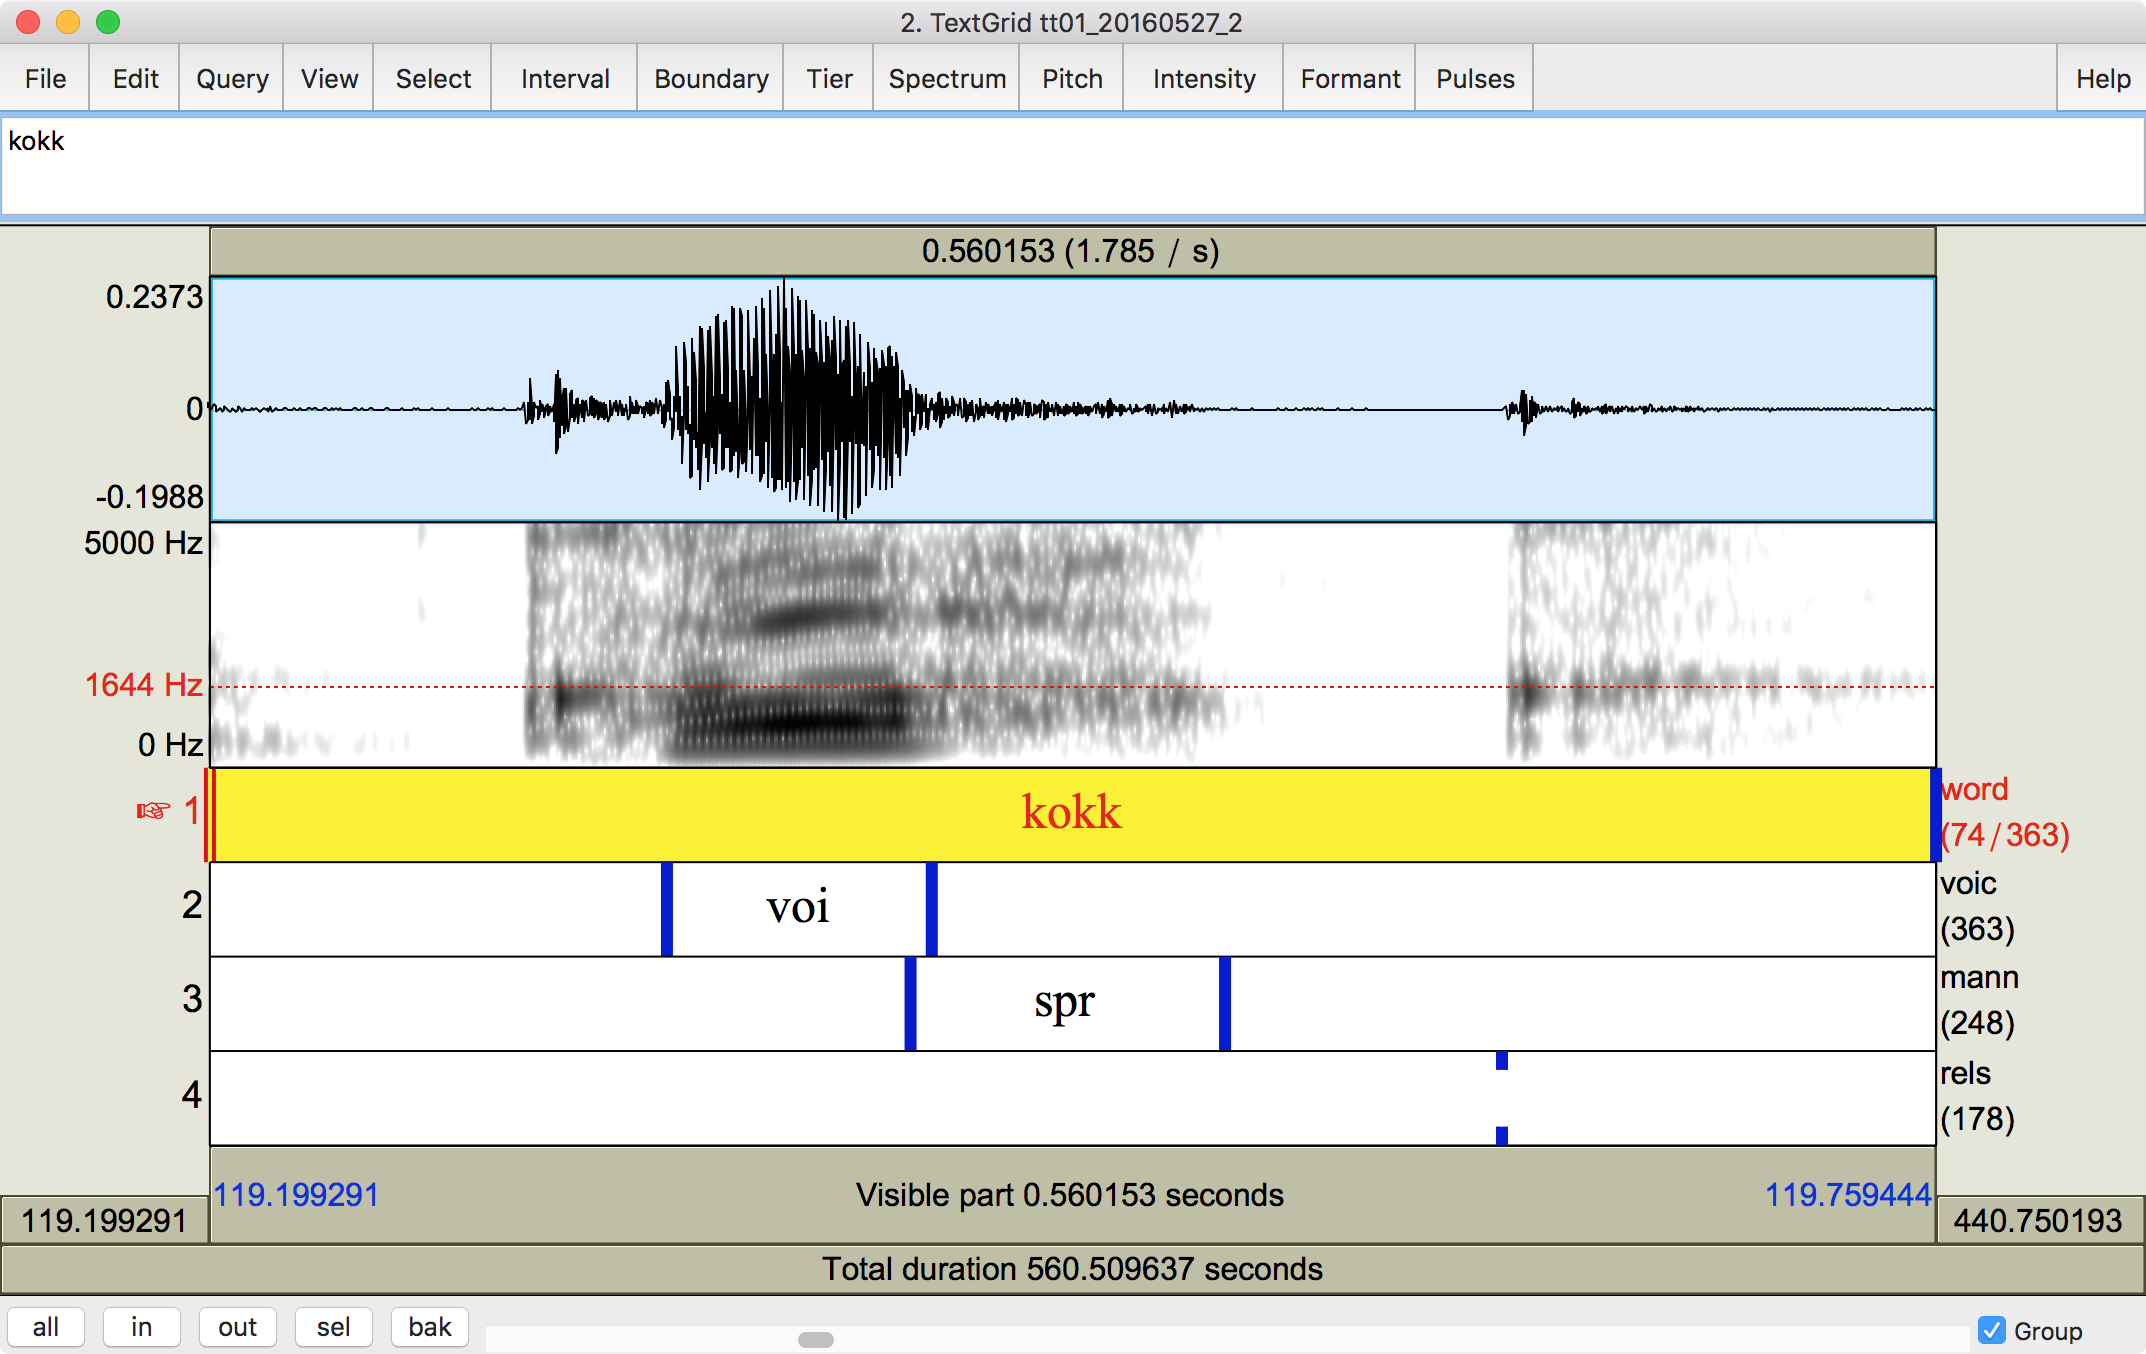
\includegraphics[width=\textwidth]{glottal}
\caption{The word \textit{kokk} `cook' as an example of the annotation of glottal spread.}
\label{f:glottal}
\end{figure}


A single tier was used to annotate glottal spread, nasal airflow, laterality and rhoticity.
Marking the beginning of glottal spread proved to be particularly difficult.
The common realisation of the combination ``vowel + pre-aspiration'' is structured as follows: the first portion of the vowel is accompanied by modal voicing; the vocal folds start moving apart from each other in an abduction gesture while they still vibrate (breathy voice); then, vocal fold vibration stops while voiceless friction remains (at the glottis or at the oral cavity, depending on the place of articulation vowel).
As \citet{khan2012} and \citet{nance2013} point out, breathy voice is expected to produce more round-shaped periodic waves.
I took the onset of such more sinusoidal waves to coincide with glottal spread and I marked it as the left boundary of the spreading gesture.
At times, however, the interpretation of the waveform was not straightforward.
In these cases, I relied on the visual make-up of the spectrogram.
According to \citealt{jones2006} (cited in \citealt[134]{nance2013}), breathy voice usually correlates with smeared off or totally absent higher formants.
This is due to the presence of high-frequency noise produced by the increased amount of airflow coming from the abducted glottis.
The right boundary was assumed to fall at the end of visible frication noise.

\subsection{Nasals, laterals and trills}

Following standard practice, I marked the beginning of nasality where a change in the shape of the waveform and in the amplitude of the spectrogram were visible.
I applied the same principle to laterals and trills.
I placed the right boundary of these intervals (nasal, lateral, trill) depending on the voicing of the segment.
The voiceless nasal, lateral and trill consonants terminate with voiceless friction (nareal, lateral or central, respectively).
The end of friction in these consonants was used as the end of the interval.
In the voiced counterparts of these, the end of voicing coincided with the right boundary.

\begin{figure}
\centering
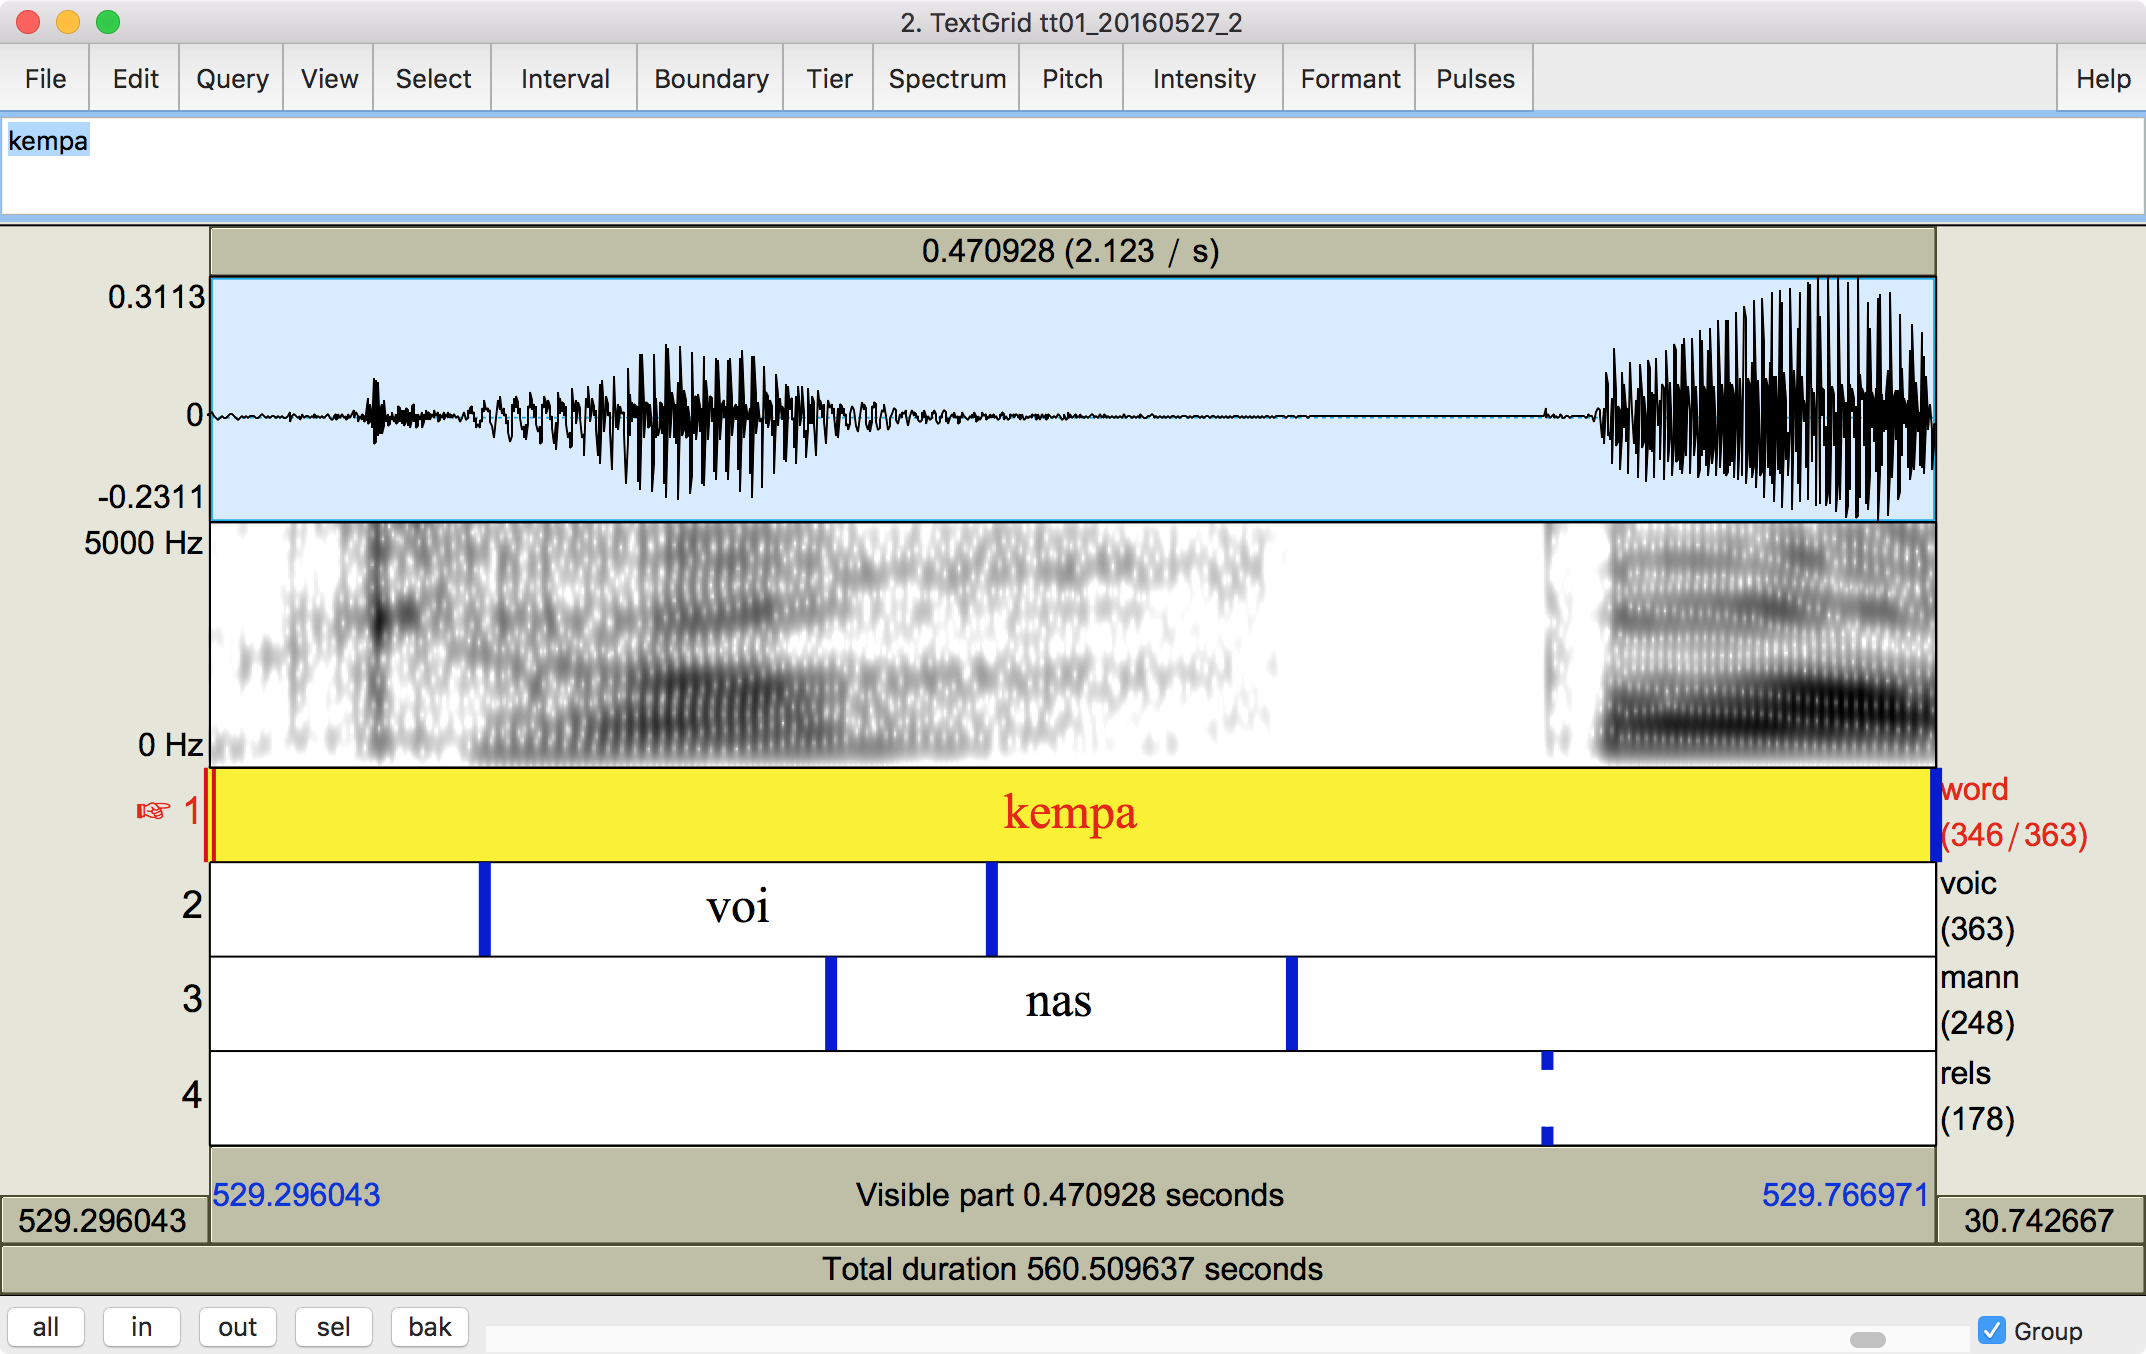
\includegraphics[width=\textwidth]{mann}
\caption{The word \textit{kempa} `hero' as an example of the annotation in the manner tier.}
\label{f:mann}
\end{figure}

\subsection{Stop release}
The last tier was dedicated to marking the consonant release of the stop following the target vowel (with or without an intervening sonorant).
The release of the stop consonant was marked at the onset of the burst.
This is normally visible on the waveform as one or more sudden peaks after the closure, or on the spectrogram as a short interval of low amplitude friction.
If the burst was not identifiable from the waveform nor from the spectrogram, no release was marked.

\begin{figure}
\centering
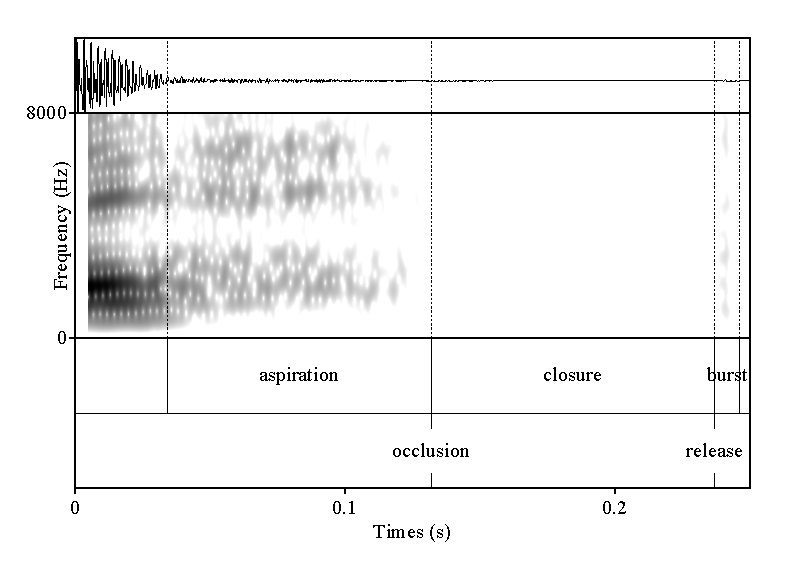
\includegraphics[width=\textwidth]{kopp}
\caption{Release of [ʰp] in the word \textit{kopp}.}
\label{f:release}
\end{figure}

\section{Measurements}
\label{s:measurements}
After the annotation was complete, I extracted the durational properties of the annotated intervals using an automated routine.
The routine was performed in PRAAT with a script, specifically written for this study.
The script with its documentation can be found in \Cref{a:getmeasure}.
The output of the extraction procedure is a \texttt{.csv} file which contains the relevant measurements.
The following measures were taken in milliseconds:

\begin{itemize}
\item \textit{Word duration}: the duration of the whole word as annotated on the word tier.
\item \textit{Duration of voicing}: the duration of the interval in the word containing vocal fold vibration (voicing tier).
\item \textit{Duration of glottal spread and consonant manner}: the duration of the portion characterised by glottal spreading, nasality, laterality or rhoticity (manner tier).
\item \textit{Duration of the vowel}.
This was measured depending on the phonological form of the word.
In words containing a pre-aspirated geminate or a sonorant (nasal, lateral or trill), as the duration of the interval between the onset of voicing and the onset of the interval on the manner tier.
In words with non-aspirated geminates, the duration of absolute voicing is equal to the duration of voicing.
\item \textit{Stop closure duration}: the duration of the closure of the stop consonant, calculated as the duration of the interval between the off-set of voicing, glottal spread or consonant manner, and the release.
\item \textit{Closure duration}: the duration of the interval between the on-set of glottal spread or consonant manner and the release; in words with non-aspirated geminates, it is equal to the stop closure duration.
\item \textit{Voice Onset to Release} (VOR): the duration of interval between the onset of voicing and the release of the stop closure.
\item \textit{Voice Offset to Release} (\textsc{VOffR}): the duration of the interval between the offset of voicing and the release of the stop closure.
\item \textit{Duration of glottal spread}. The duration of the interval calculated as the duration of spreading in stops and from the offset of voicing to the offset of manner in sonorants.
\end{itemize}

To control for differences in speech rate, I opted to normalise the measurements.
Normalisation was achieved by dividing the relevant measure by the VOR.
This operation results in a transformation from durations in milliseconds to ratios in percentages.
I chose to use the VOR as the base for normalisation since this can be measured consistently across different word forms.
Since the word list contained monosyllabic and disyllabic words, and both classes had either consonant-initial or vowel-initial words, the VOR is the only portion that constantly contains three segments (VCC, VʰC, VRC, where ``R'' is any sonorant).\footnote{Pre-aspirated stops are phonologically geminates.}

\section{Statistical analysis}
\label{s:stats}
I carried out the statistical analysis using the R programming language \citep{r-core-team2015} in RStudio \citep{rstudio-team2015}.
I performed independent sample two-tailed \textit{t}-tests on parametric data and Wilcoxon tests on non-parametric data.
Normality was checked through Shapiro tests for normality.
The R code used in the analysis is available at this address [...].
%TODO add address!













\chapter{Results}
\label{c:results}

\section{Word duration}

The word list used in the reading task contains both mono- and disyllabic words.
Both classes are further divided between consonant- and vowel-initial words.
It is thus sensible to report some of the measures for each class separately.
The mean duration of CVCC words is 441.36 msec (SD = 78.24), while for VCC is 338.71 msec (SD = 54.86).
CVCCV words have a mean duration of 487.25 msec (SD = 59.94), while VCCV are on average 424.99 msec long (SD = 53.42).

\begin{figure}
\centering
\begin{knitrout}
\definecolor{shadecolor}{rgb}{0.969, 0.969, 0.969}\color{fgcolor}
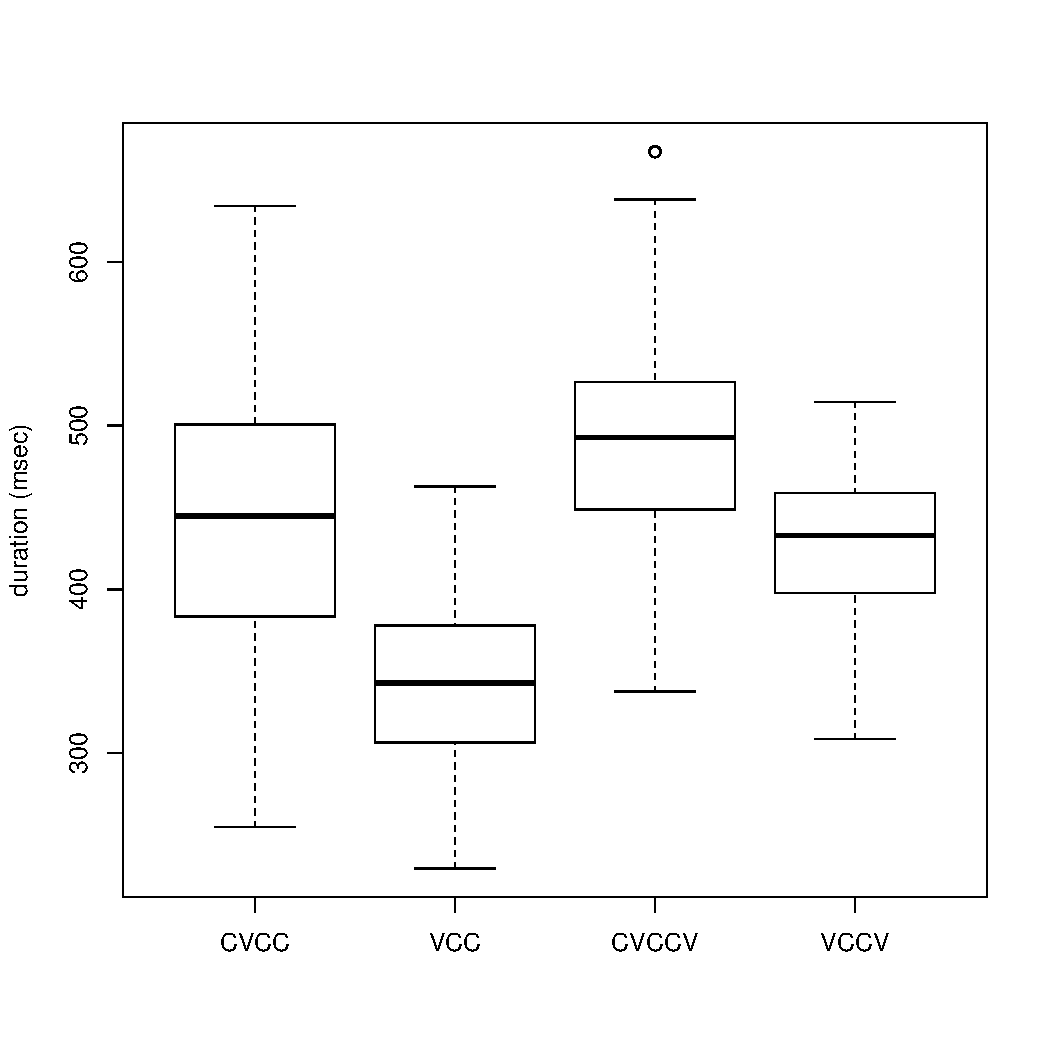
\includegraphics[width=0.8\textwidth]{img/word-duration-1} 

\end{knitrout}
\caption{Duration (in msec) of CVCC, VCC, CVCCV, and VCCV words.}
\label{f:worddur}
\end{figure}



% normalised voic is not different, but absolute is!, given that VOR is different, treat them differently
The ratio duration of the vowel was not affected by the the number of syllables of the word.
The boxplot in \Cref{f:vvpsyll} shows the duration of the vowel in milliseconds.
According to a two-sample Wilcoxon test, the mean duration of the vowel in monosyllabic words (88.67) does not differ significantly from the mean duration in disyllabic words (84.21) [V = 35302, p < 0.001].
%However, the voice on-set to release was shorter in disyllabic words () than in monosyllabic words () [].
%% kembt behave strange, in bte
%Since duration normalisation was based on the voice on-set to release duration, in the next sections I will discuss monosyllabic and disyllabic words separately.

\begin{figure}
\centering
\begin{knitrout}
\definecolor{shadecolor}{rgb}{0.969, 0.969, 0.969}\color{fgcolor}
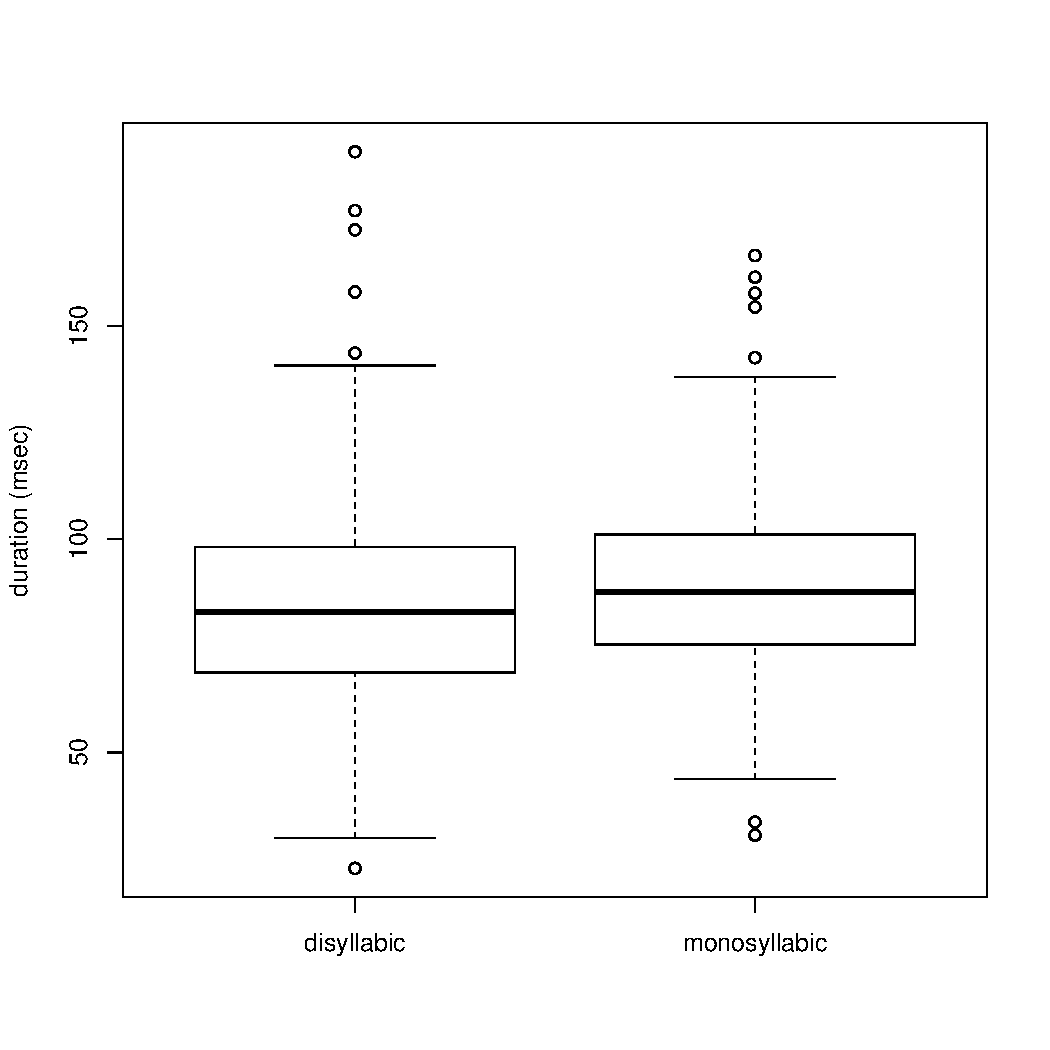
\includegraphics[width=0.8\textwidth]{img/voic-syll-box-1} 

\end{knitrout}
\caption{Vowel duration in monosyllabic vs. disyllabic words.}
\label{f:vvpsyll}
\end{figure}

\section{Voice onset to release (VOR)}



The Voice onset to Release (VOR) measures the interval between the voice onset of the critical syllable to the release of the next consonant.
According to tests for the difference between means, the VOR in all classes of words, except for -VCC words, did not have a significant difference in mean duration in both the non-aspirated and aspirated condition.

%TODO table with mean and sd

%\ctable[caption = Means and standard deviations of VOR in each word class.,
%label = t:vor
%]{lrr}{}{
%\FL

%}


\begin{figure}
\begin{subfigure}{.5\textwidth}
\centering
\begin{knitrout}
\definecolor{shadecolor}{rgb}{0.969, 0.969, 0.969}\color{fgcolor}
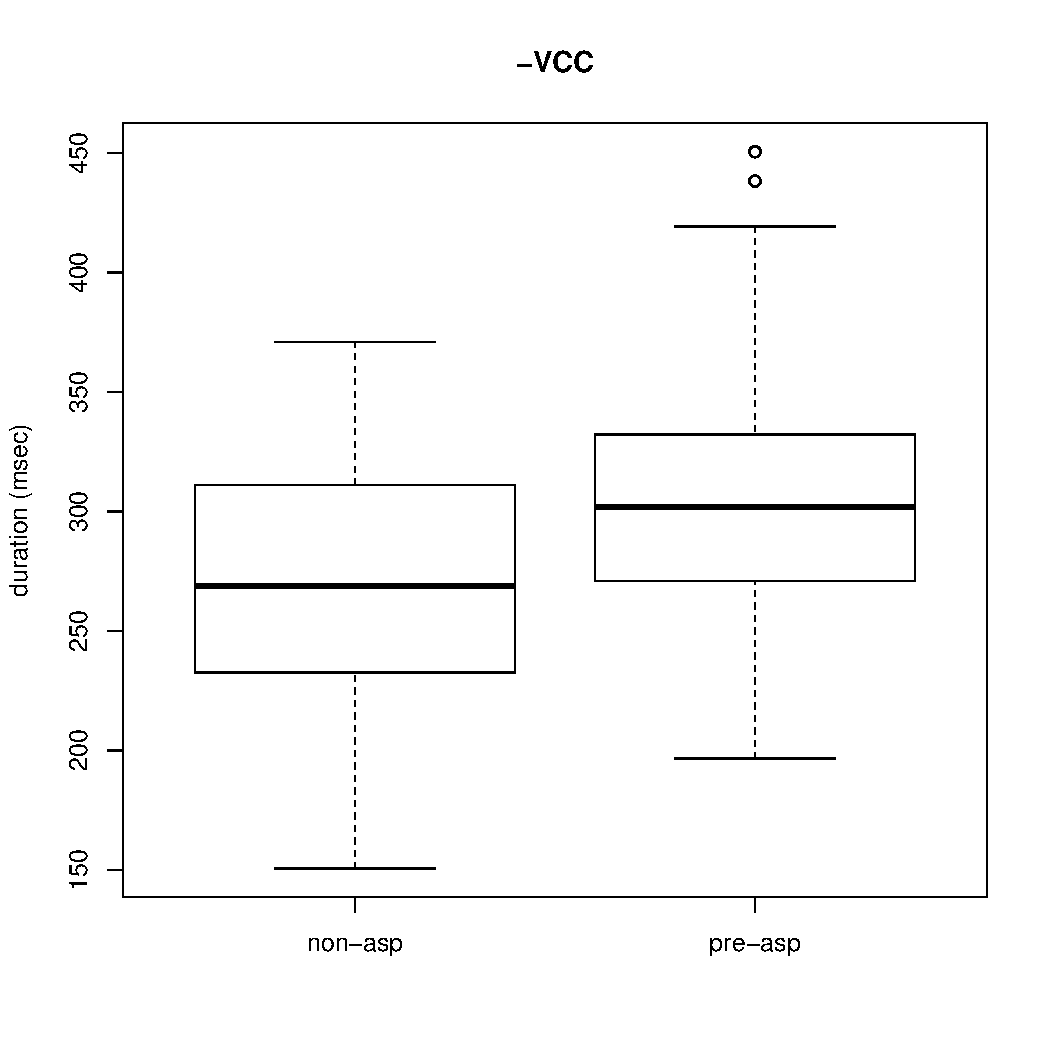
\includegraphics[width=\textwidth]{img/mono-stop-vor-1} 

\end{knitrout}
\end{subfigure}
\begin{subfigure}{.5\textwidth}
\centering
\begin{knitrout}
\definecolor{shadecolor}{rgb}{0.969, 0.969, 0.969}\color{fgcolor}
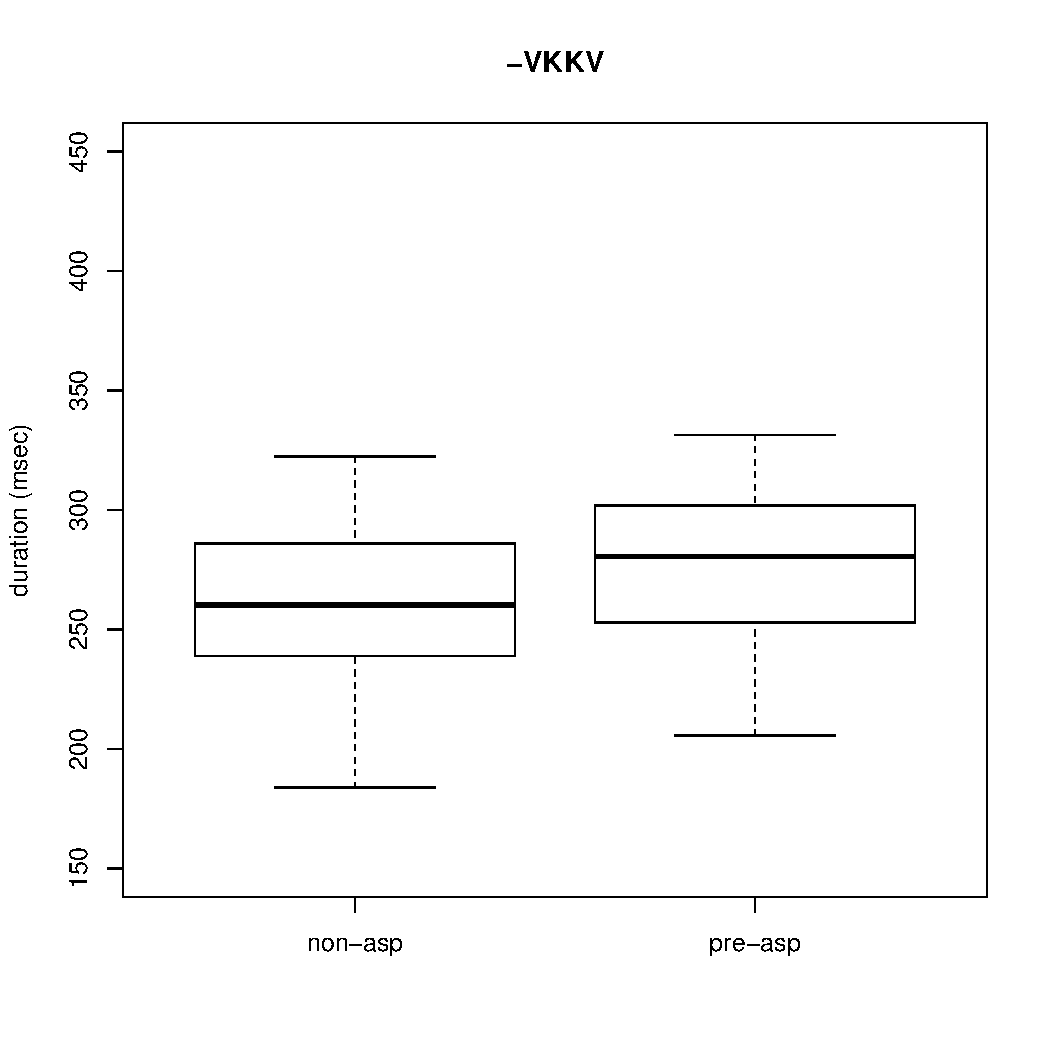
\includegraphics[width=\textwidth]{img/di-stop-vor-1} 

\end{knitrout}
\end{subfigure}
\begin{subfigure}{.5\textwidth}
\centering
\begin{knitrout}
\definecolor{shadecolor}{rgb}{0.969, 0.969, 0.969}\color{fgcolor}
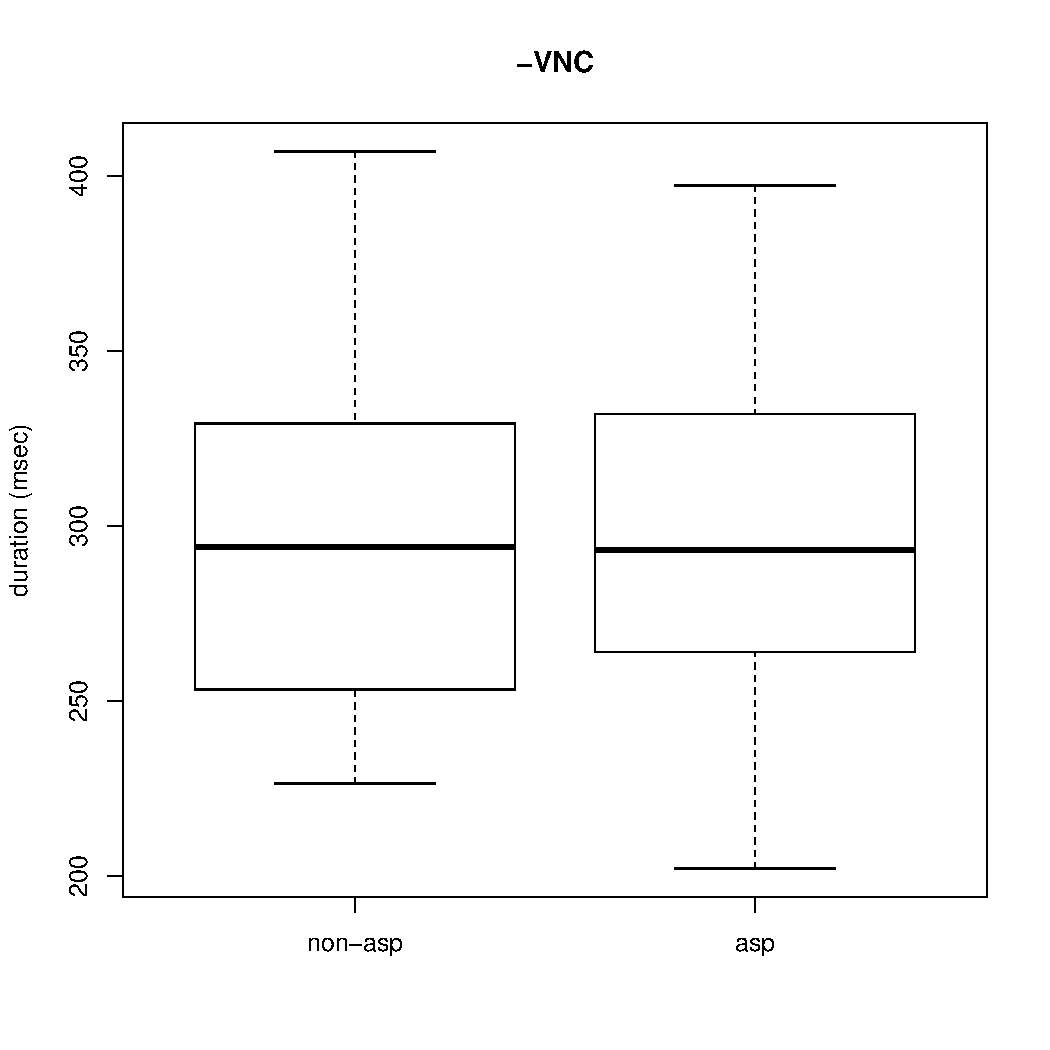
\includegraphics[width=\textwidth]{img/mono-nas-vor-1} 

\end{knitrout}
\end{subfigure}
\begin{subfigure}{.5\textwidth}
\centering
\begin{knitrout}
\definecolor{shadecolor}{rgb}{0.969, 0.969, 0.969}\color{fgcolor}
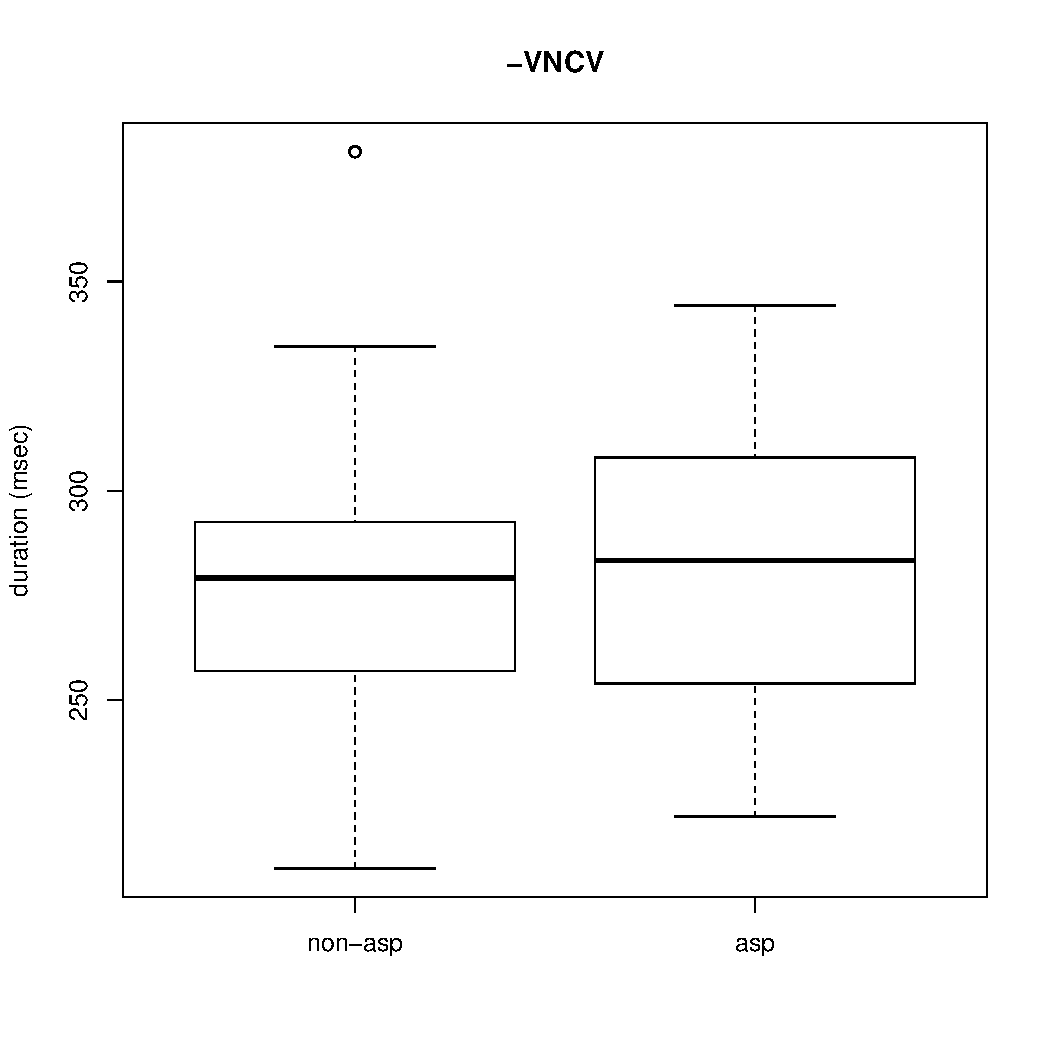
\includegraphics[width=\textwidth]{img/di-nas-vor-1} 

\end{knitrout}
\end{subfigure}
\begin{subfigure}{.5\textwidth}
\centering
\begin{knitrout}
\definecolor{shadecolor}{rgb}{0.969, 0.969, 0.969}\color{fgcolor}
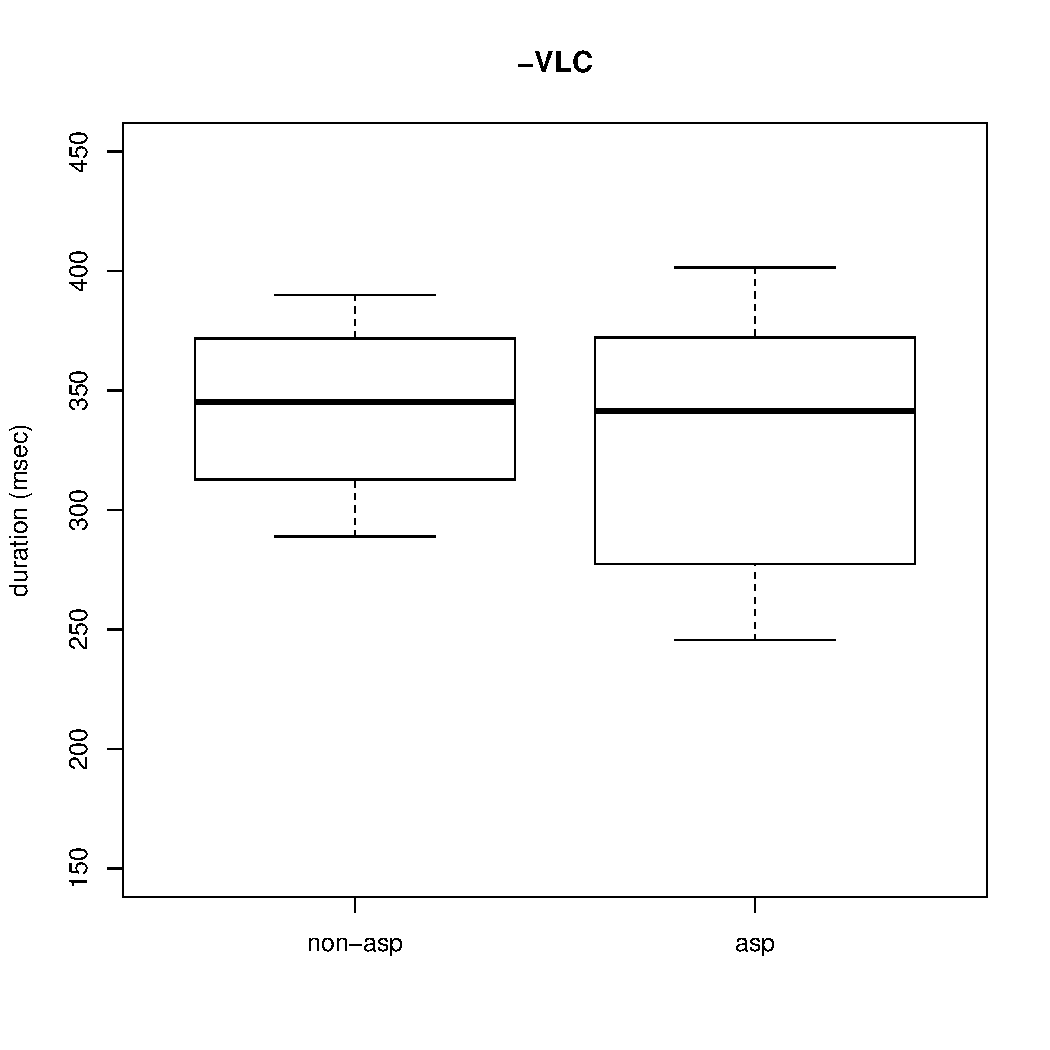
\includegraphics[width=\textwidth]{img/mono-lat-vor-1} 

\end{knitrout}
\end{subfigure}
\begin{subfigure}{.5\textwidth}
\centering
\begin{knitrout}
\definecolor{shadecolor}{rgb}{0.969, 0.969, 0.969}\color{fgcolor}
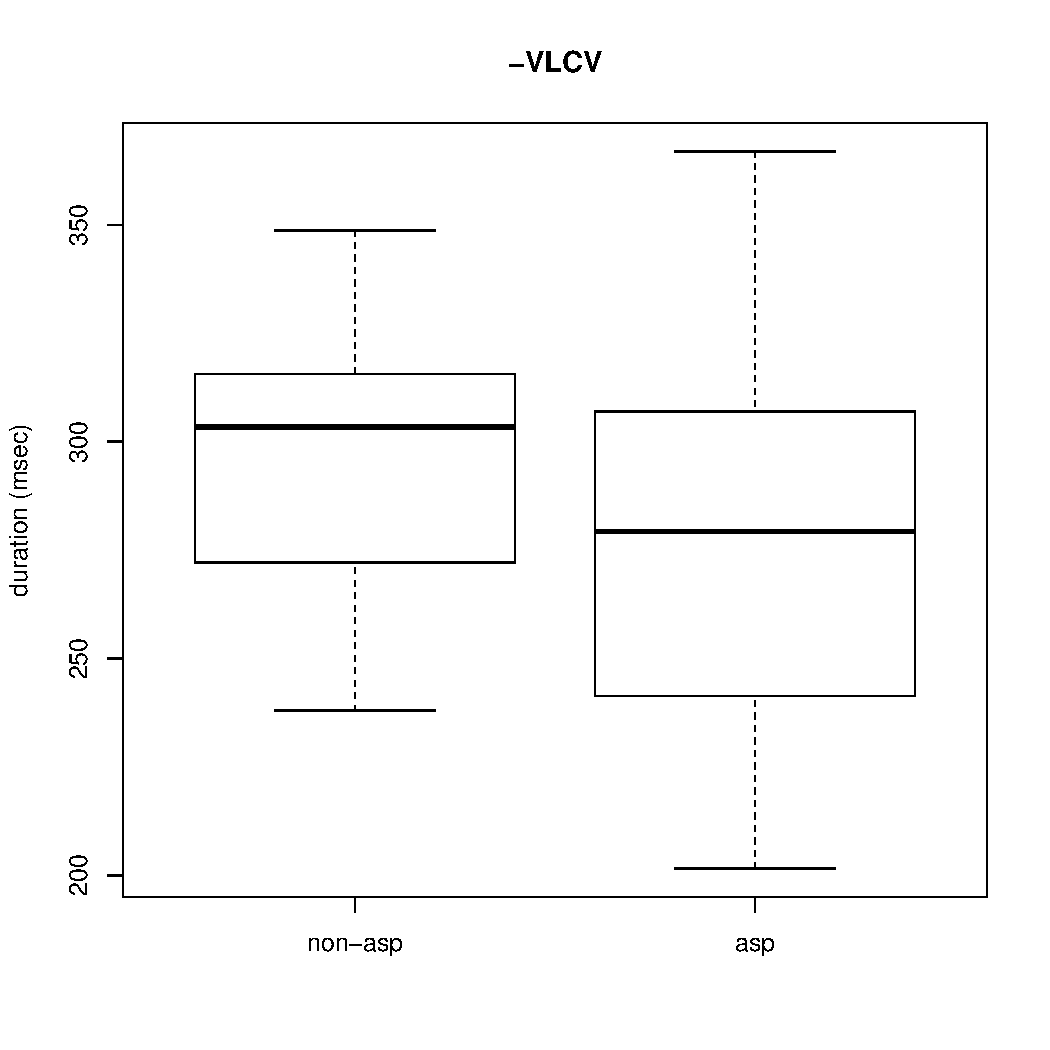
\includegraphics[width=\textwidth]{img/di-lat-vor-1} 

\end{knitrout}
\end{subfigure}
\caption{Duration (in msec) of the Voice Onset to Release (VOR).}
\label{f:vor}
\end{figure}

\begin{figure}
\centering
\begin{knitrout}
\definecolor{shadecolor}{rgb}{0.969, 0.969, 0.969}\color{fgcolor}
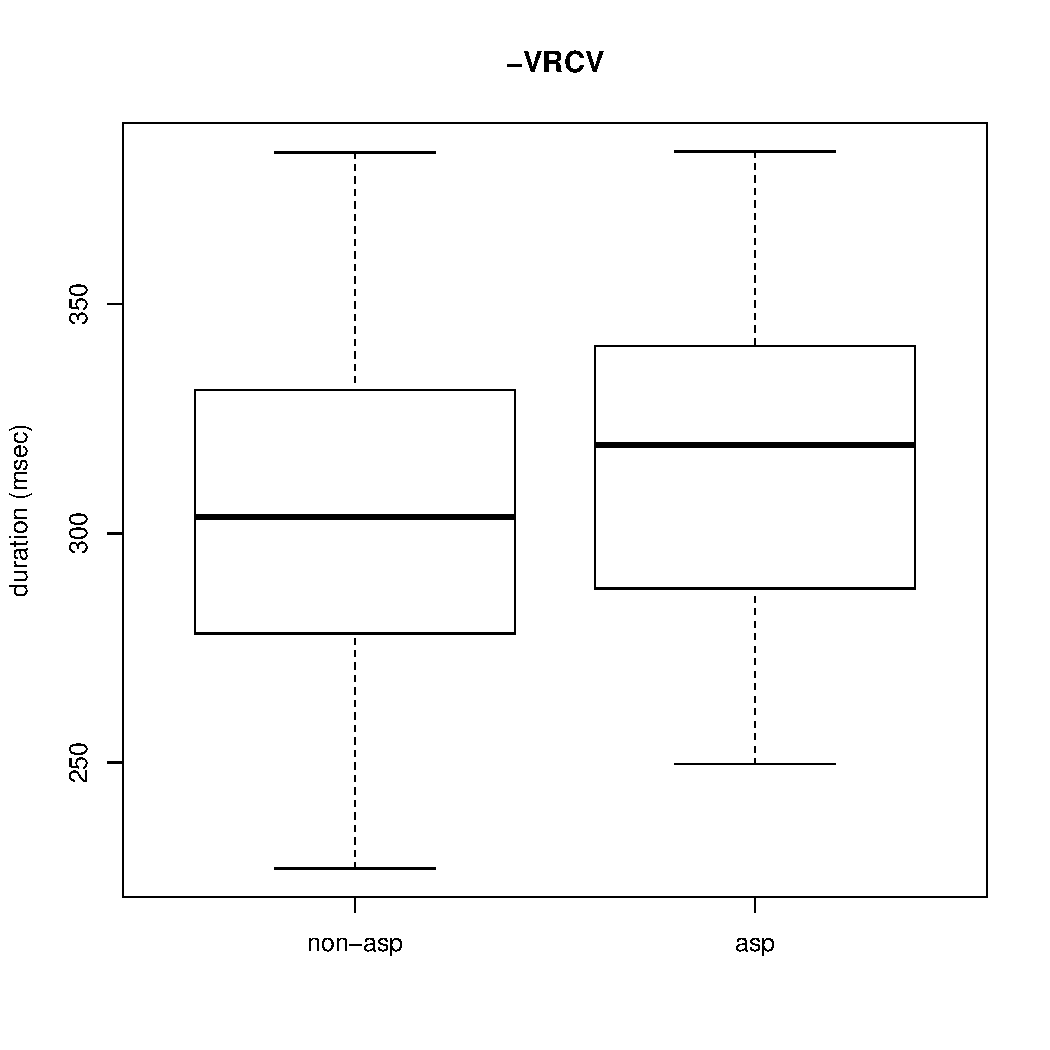
\includegraphics[width=0.8\textwidth]{img/di-rho-vor-1} 

\end{knitrout}
\caption{Duration (in msec) of the Voice Onset to Release (VOR) of VRCV words.}
\label{f:vor-rho}
\end{figure}


\section{Vowel duration}
\label{s:vow-dur}

\subsection{Geminate stops}


The mean duration of vowels in milliseconds was 98 (SD = 19.1) in monosyllabic words ending in a non-aspirated geminate stop, while it was 84.47 (SD = 22.71) if followed by a pre-aspirated geminate stop.
\Cref{f:monostop} shows the ratio duration of the vowel in the two conditions.
The difference in the mean of the vowel ratio between the non-aspirated (0.37, SD = 0.07) and the aspirated class of words (0.28, SD = 0.05) was significant [W = 7793, p-value < 0.001].

\begin{figure}
\begin{subfigure}{.5\textwidth}
\centering
\begin{knitrout}
\definecolor{shadecolor}{rgb}{0.969, 0.969, 0.969}\color{fgcolor}
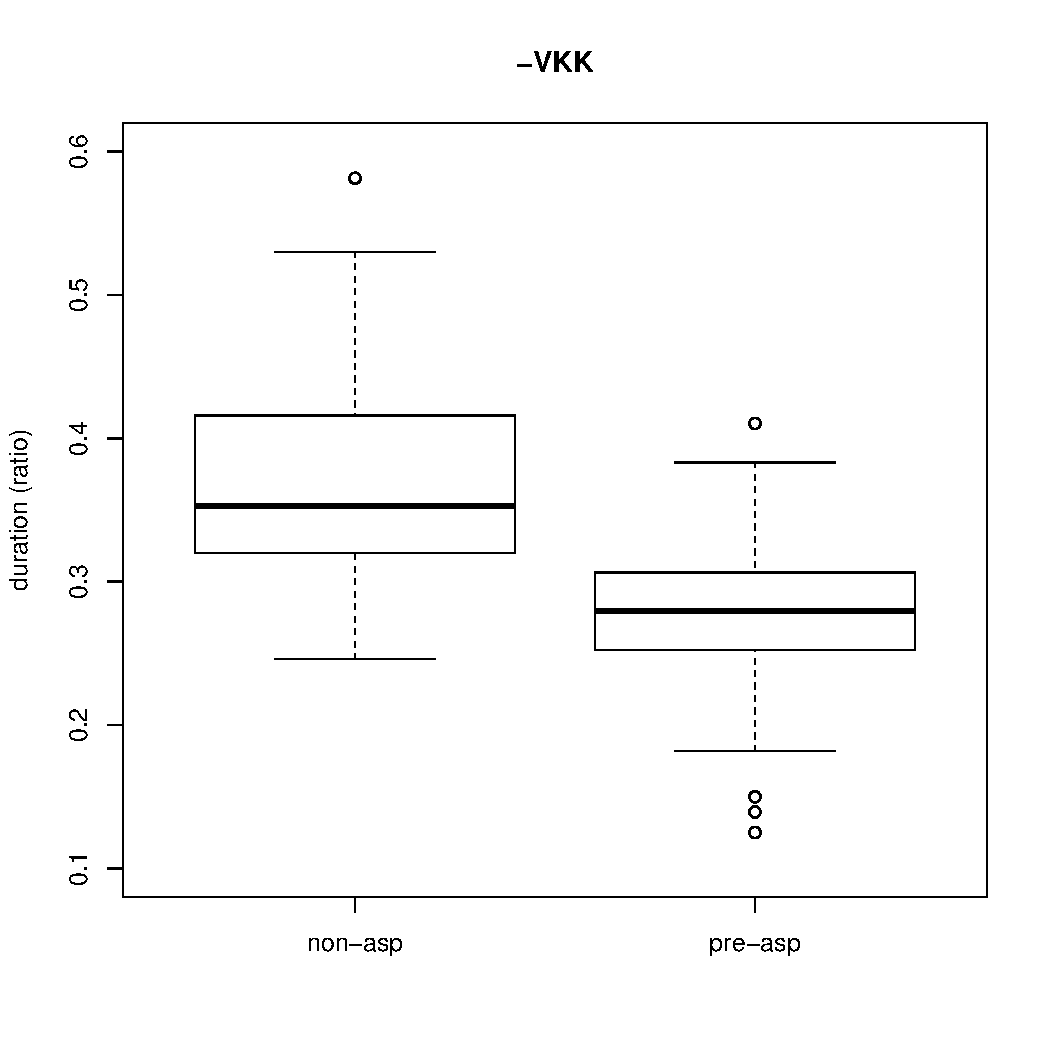
\includegraphics[width=\textwidth]{img/mono-stop-box-1} 

\end{knitrout}
\label{f:monostop}
\end{subfigure}
\begin{subfigure}{.5\textwidth}
\centering
\begin{knitrout}
\definecolor{shadecolor}{rgb}{0.969, 0.969, 0.969}\color{fgcolor}
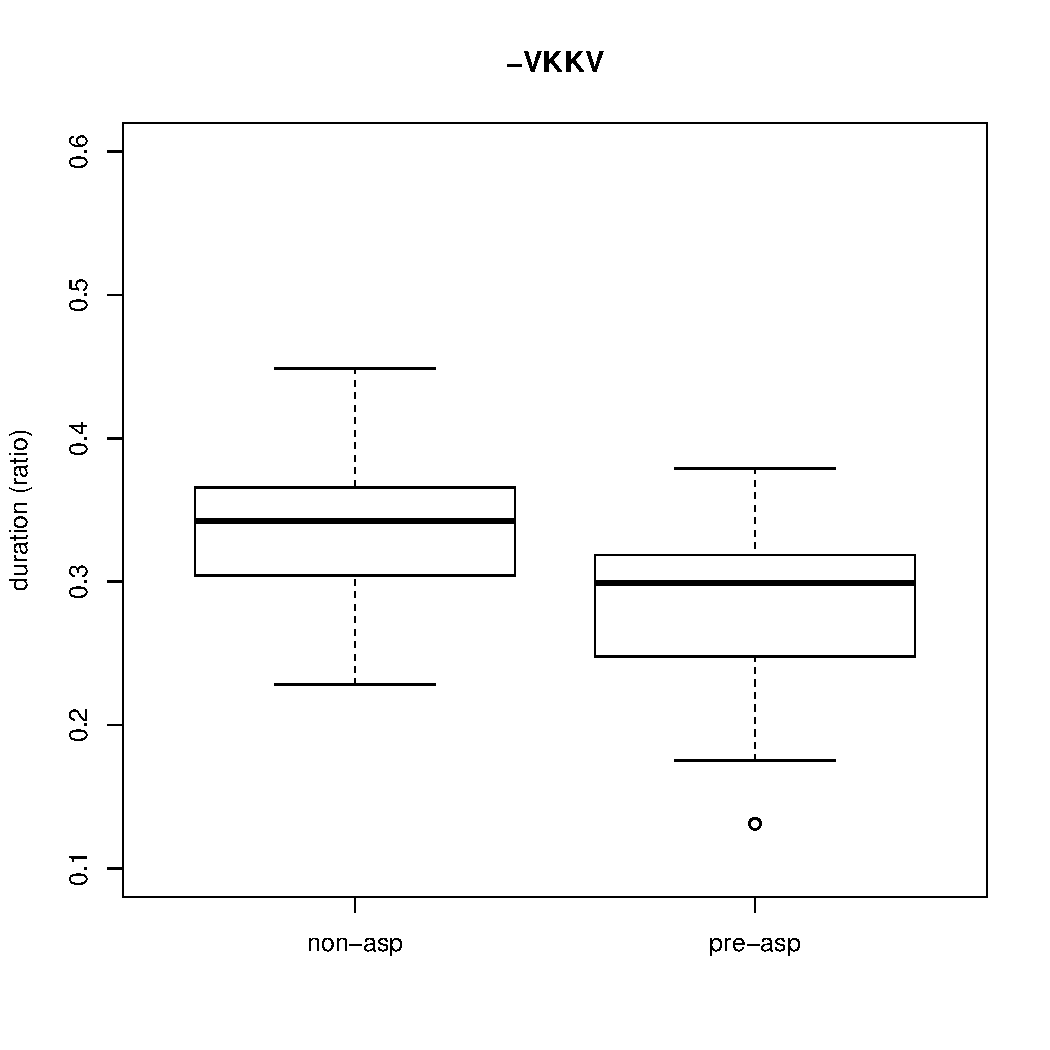
\includegraphics[width=\textwidth]{img/di-stop-box-1} 

\end{knitrout}
\end{subfigure}
\begin{subfigure}{.5\textwidth}
\centering
\begin{knitrout}
\definecolor{shadecolor}{rgb}{0.969, 0.969, 0.969}\color{fgcolor}
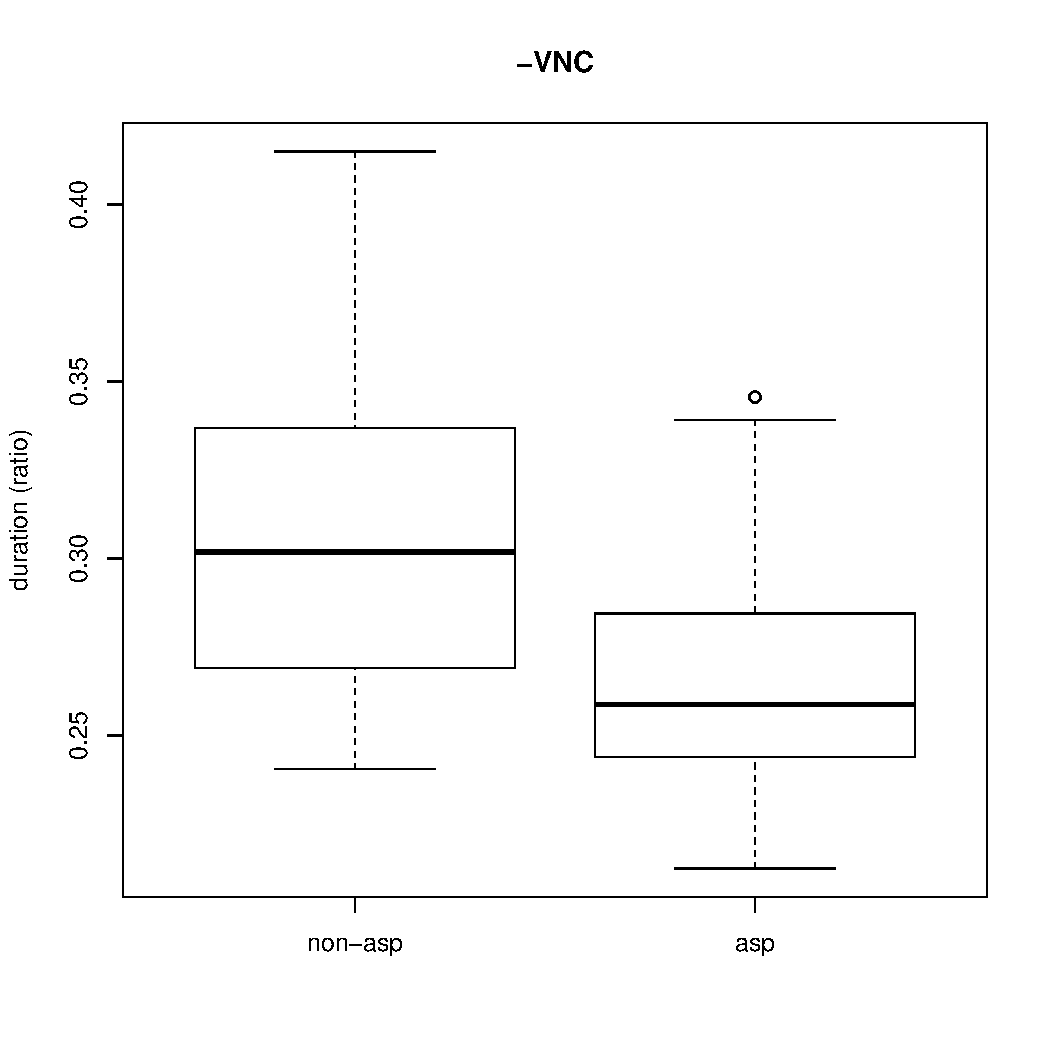
\includegraphics[width=\textwidth]{img/mono-nas-box-1} 

\end{knitrout}
\end{subfigure}
\begin{subfigure}{.5\textwidth}
\centering
\begin{knitrout}
\definecolor{shadecolor}{rgb}{0.969, 0.969, 0.969}\color{fgcolor}
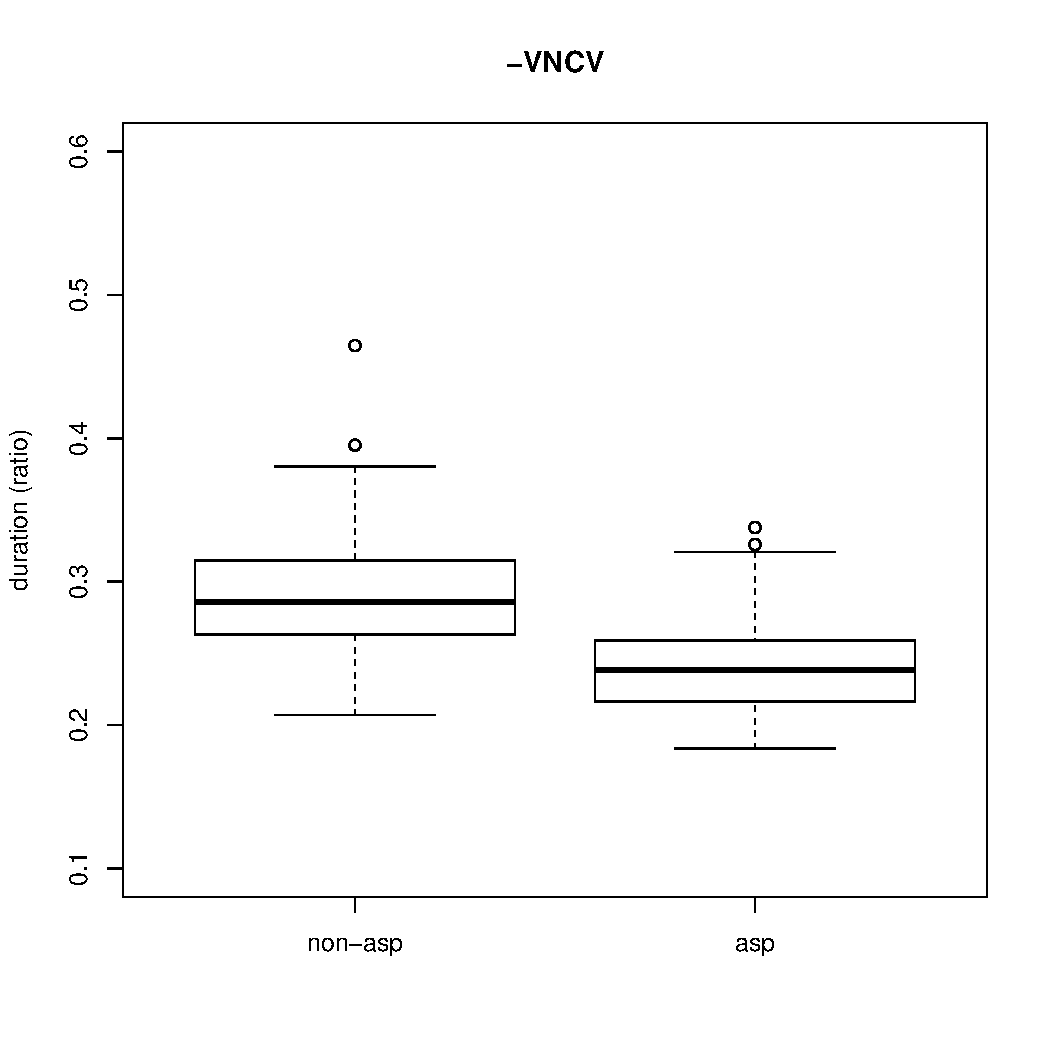
\includegraphics[width=\textwidth]{img/di-nas-box-1} 

\end{knitrout}
\end{subfigure}
\begin{subfigure}{.5\textwidth}
\centering
\begin{knitrout}
\definecolor{shadecolor}{rgb}{0.969, 0.969, 0.969}\color{fgcolor}
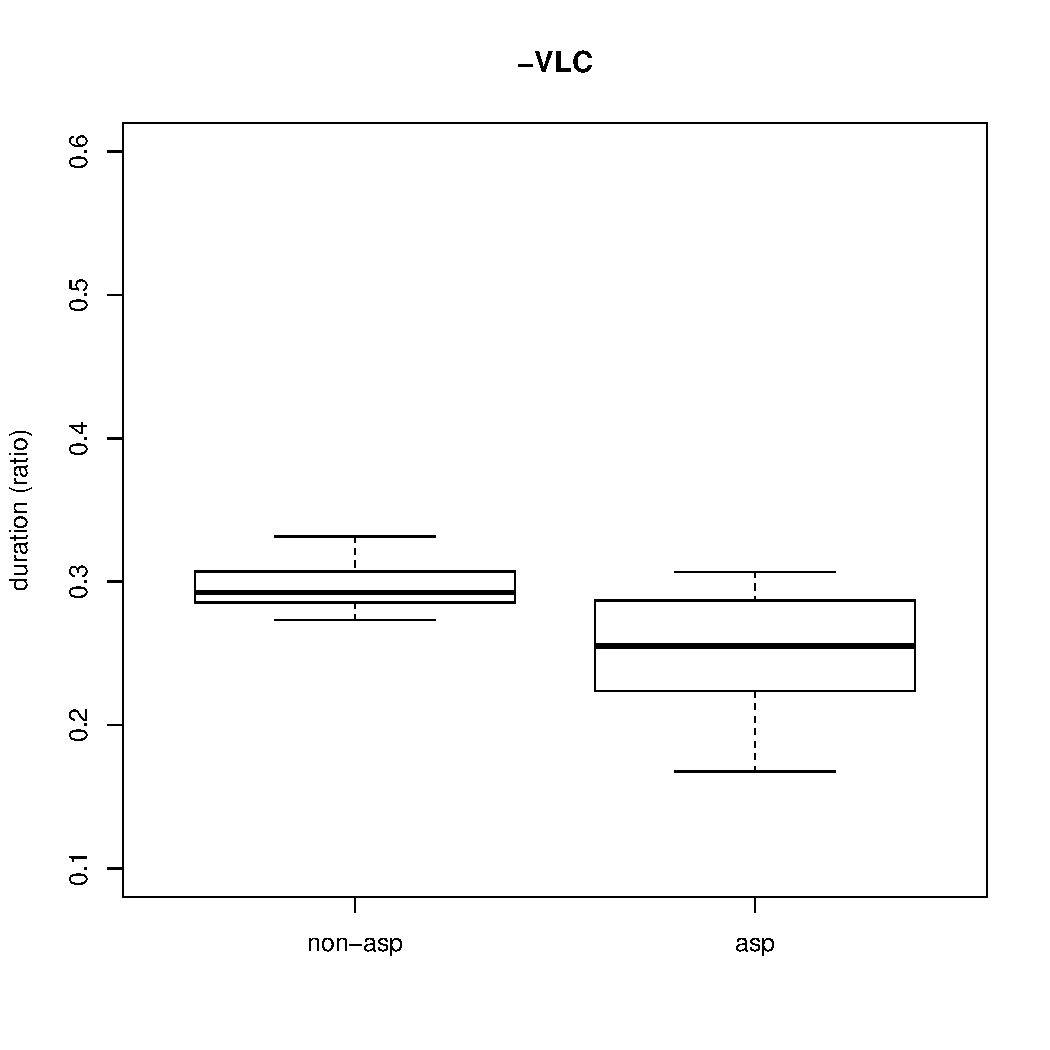
\includegraphics[width=\textwidth]{img/mono-lat-box-1} 

\end{knitrout}
\end{subfigure}
\begin{subfigure}{.5\textwidth}
\centering
\begin{knitrout}
\definecolor{shadecolor}{rgb}{0.969, 0.969, 0.969}\color{fgcolor}
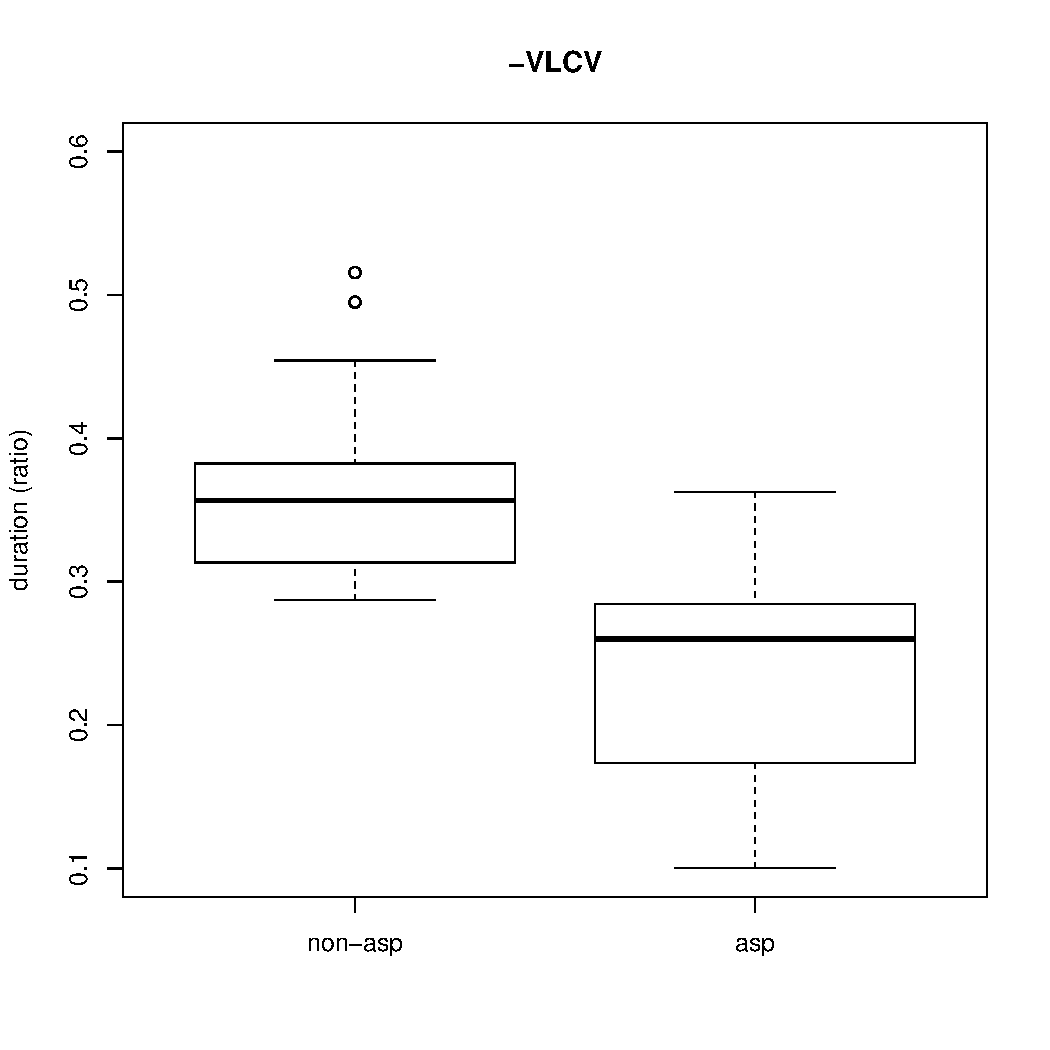
\includegraphics[width=\textwidth]{img/di-lat-box-1} 

\end{knitrout}
\end{subfigure}
\caption{Vowel duration (ratio) depending on the presence \textit{vs}. absence of pre-aspiration in the following consonant}
\label{f:vowelduration}
\end{figure}

\begin{figure}
\centering
\begin{knitrout}
\definecolor{shadecolor}{rgb}{0.969, 0.969, 0.969}\color{fgcolor}
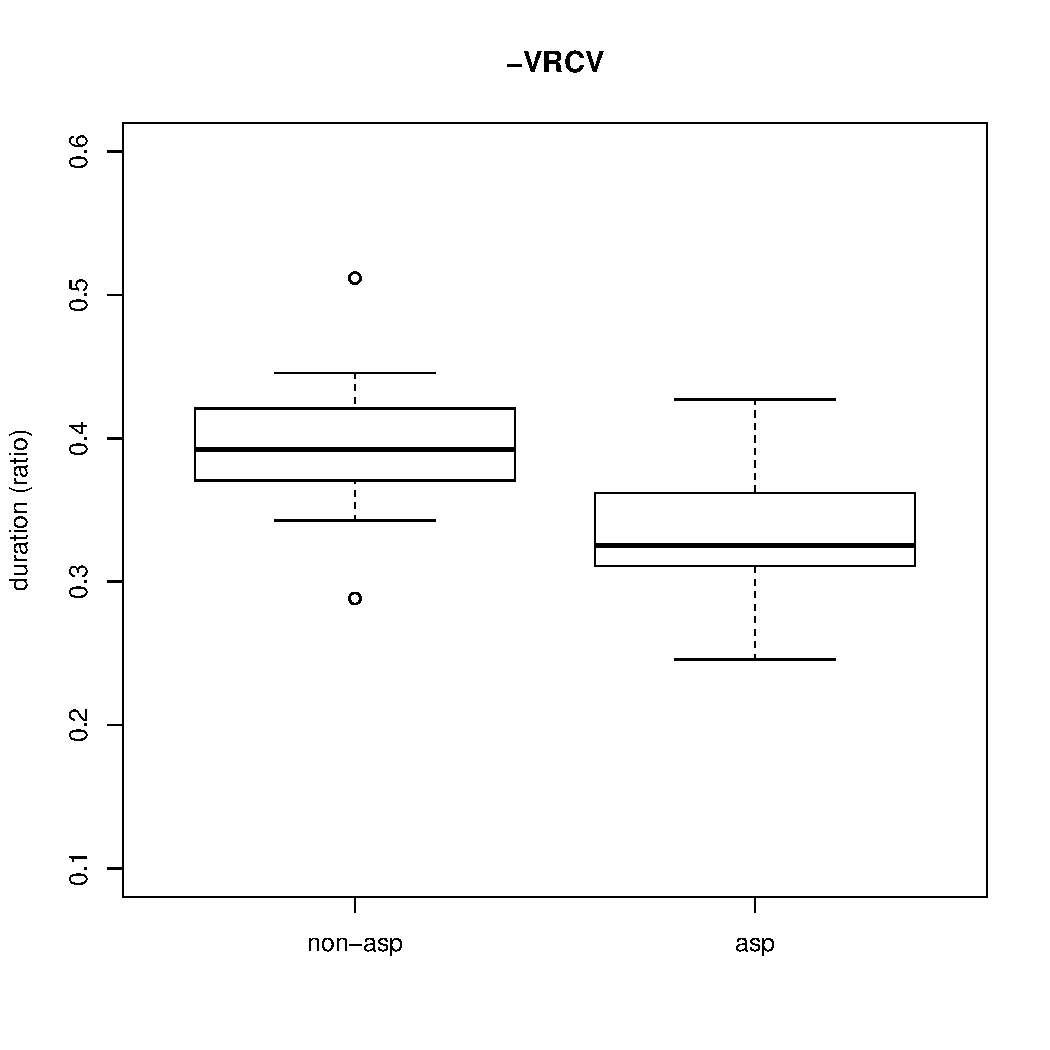
\includegraphics[width=0.8\textwidth]{img/di-rho-box-1} 

\end{knitrout}
\caption{Ratio vowel duration in words with an /rC/ cluster.}
\label{f:voweldurrho}
\end{figure}



In disyllabic words, the voiced vocalic portion is 86.97 (SD = 13.28) msec long if followed by a non-aspirated geminate, and 78.04 (SD = 20.53)msec long if followed by a pre-aspirated geminate.
In ratio terms, the voiced part makes up the 33.61\% (SD = 0.05) of the VOR in word with plain geminates, and the 28.27\% (SD = 20.53) in words with pre-aspirated geminates.
According to a independent two-sample \textit{t}-test, the difference in ratio is significant [t = 4.39, df = 50.46, p < 0.001].

\subsection{Nasals}


Words of the form (C)VNC showed a mean voiced portion duration of 89.96 msec if the nasal is voiced and 77.73 msec if voiceless.
The normalised duration was, respectively, 0.31 (SD = 0.05) and 0.26 (SD = 0.03).
The difference in ratio duration was significant [W = 836, p < 0.001].



CVNCV words have a mean voiced vocalic portion duration of 81.72 msec (SD = 17.66) if the nasal is voiced and 67.48 msec  (SD = 0.03) if it is voiceless.
As percentages, the vocalic portion is 29.47\% of the VOR if followed by a voiced nasal, and 24.16\% when the nasal is voiceless.
A \textit{t}-test showed that this difference is significant [t = 7.04, df = 119.99, p < 0.001].


\subsection{Laterals}


In the case of words ending in a /lC/ cluster, the mean duration of the vocalic portion were 102.05 (SD = 11.77) and 80.7 msec (SD = 13.02) when followed, respectively by a voiced and voiceless lateral.
These correspond to the 29.69\% and the 24.98\% of the VOR.
A t-test shows that the difference is significant [t = 4.1, df = 20.43, p < 0.001].




The voiced vocalic portion in CVLCV words is on average 107.68 msec long (SD = 22.78) when the lateral is voiced and 66.66 msec (SD = 0.07) when it is voiceless.
The voiced portion takes the 36.2\% of the VOR if followed by a voiced lateral, and 23.26\% when the lateral is voiceless.
A t-test reveals the difference to be significant [t = 7.47, df = 50.72, p < 0.001].

\subsection{Rhotics}



With words containing an /rC/ cluster, the mean duration of the voiced vocalic portion is 121.07 msec long (SD = 0.05) when the rhotic is voiced and 104.78 msec (SD = 0.05) when it is voiceless.
The voiced portion takes the 39.83\% of the VOR if followed by a voiced rhotic, and 33.43\% when the rhotic is voiceless.
A t-test gave a significant result [t = 3.4, df = 27.98, p < 0.001].

\section{Duration of stop closure}


The ratio duration of stop closure in words containing a sonorant + stop cluster was not significantly different in the non-aspirated and aspirated condition, except in disyllabic words with an /lC/ [t = 2.51, df = 54.7, p < 0.001] and /rC/ cluster [t = 5.62, df = 27.82, p < 0.001].
Unsurprisingly, the duration of stop closure in words with geminate stops was significantly different in the two conditions, since pre-aspirated stops have a later closure.

\begin{figure}
\centering
\begin{knitrout}
\definecolor{shadecolor}{rgb}{0.969, 0.969, 0.969}\color{fgcolor}
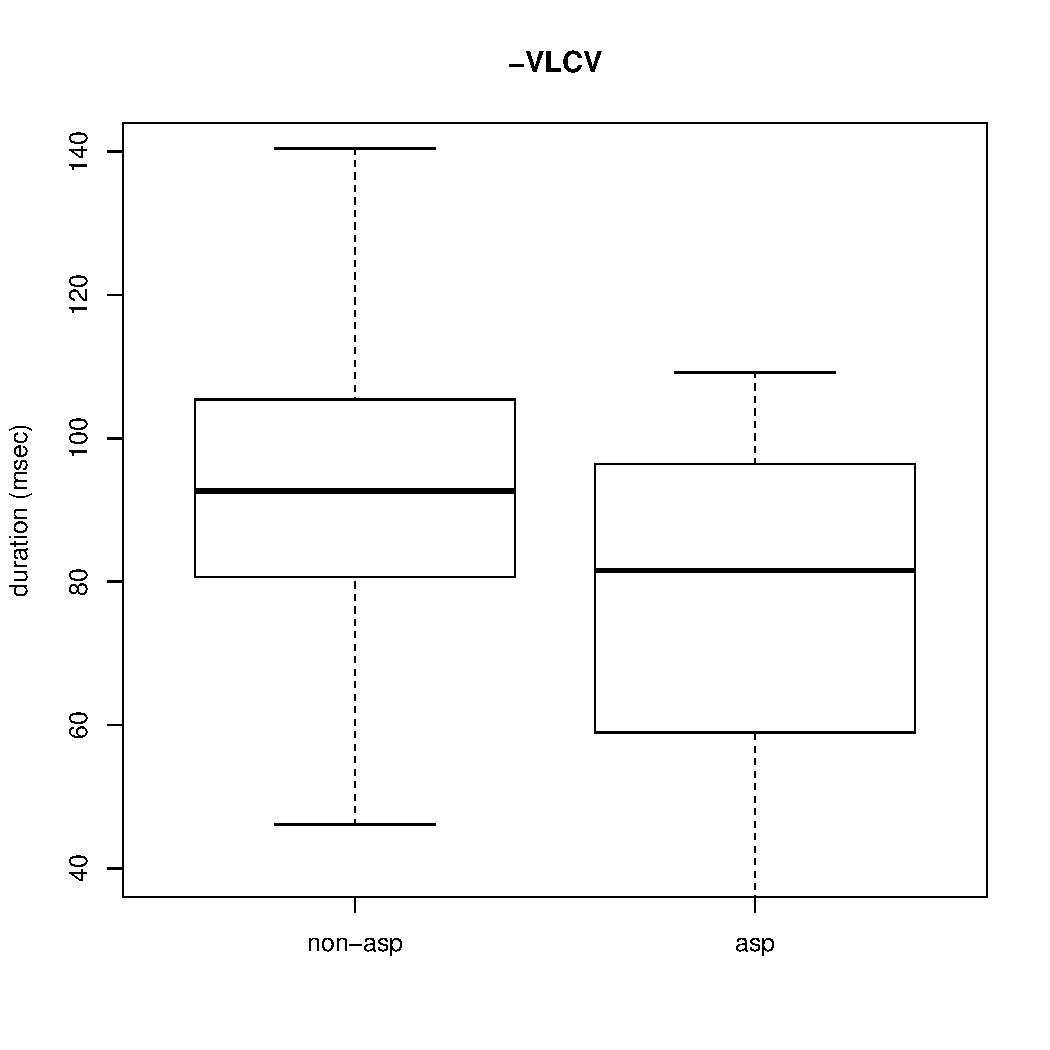
\includegraphics[width=0.8\textwidth]{img/di-lat-clos-box-1} 

\end{knitrout}
\caption{Stop closure duration (msec) in -LCV words.}
\label{f:dilatclos}
\end{figure}

\begin{figure}
\centering
\begin{knitrout}
\definecolor{shadecolor}{rgb}{0.969, 0.969, 0.969}\color{fgcolor}
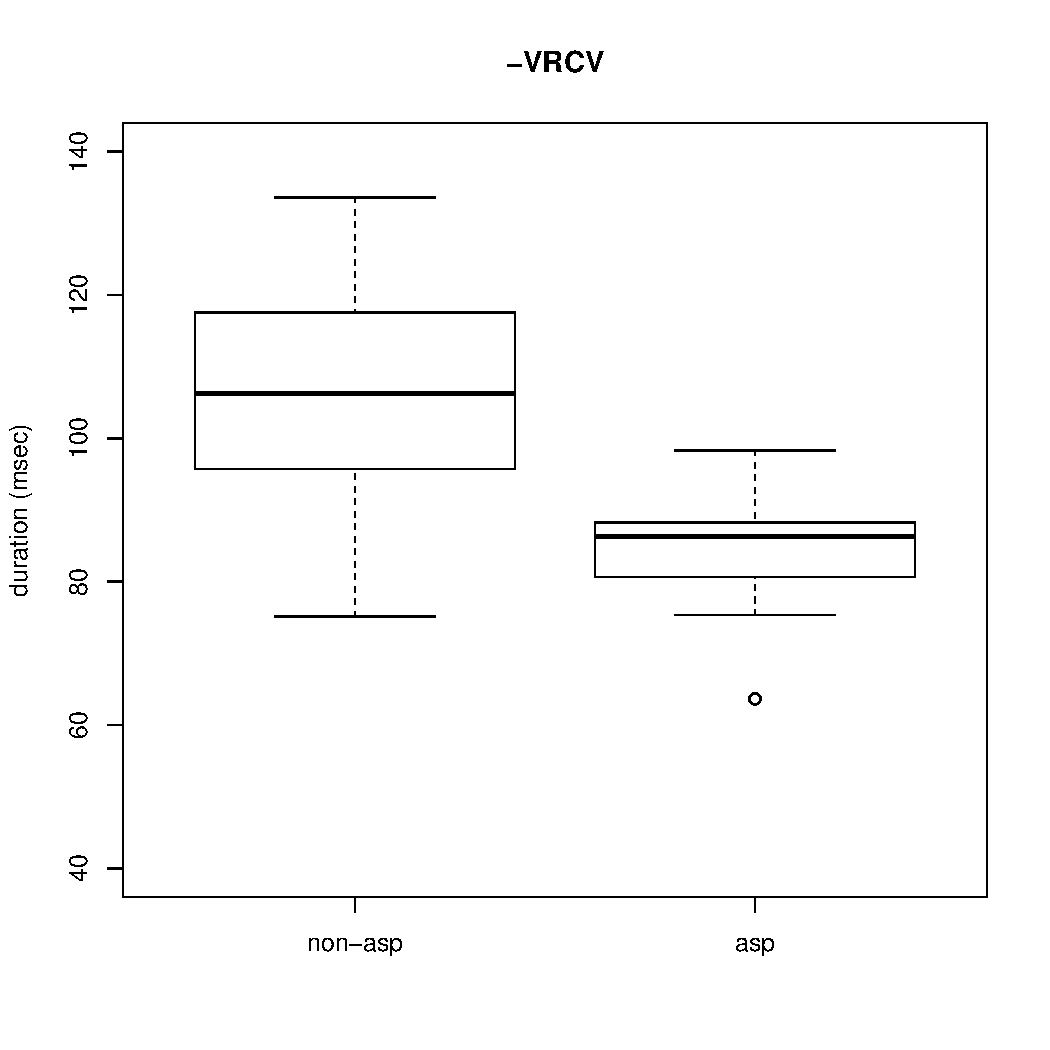
\includegraphics[width=0.8\textwidth]{img/di-rho-clos-box-1} 

\end{knitrout}
\caption{Stop closure duration (msec) in VRCV words.}
\label{f:dirhoclos}
\end{figure}

\section{Duration of glottal spread}
\label{s:gs}


The duration of glottal spread was measured as the duration of vocal folds abduction in stops and as the duration of the voiceless portion in sonorants.
According to a Kruskal-Wallis rank sum test, the duration of glottal spread in the stop, nasal, lateral and trill classes are different as the level of significance [Kruskal-Wallis $\chi^2$ = 44.11, df = 3, p < 0.001].
A post-hoc Games-Howell test for unequal variances showed that, while the duration of the spreading gesture did not differ between laterals, trilss and stops, the duration of glottal abduction in nasals was significantly different from that one in laterals [t = 3.79, df = 75.99, p = 0.002] and stops [t = 6.53, df = 137.2, p < 0.001] (but not from the one in trills).

\begin{figure}
\centering
\begin{knitrout}
\definecolor{shadecolor}{rgb}{0.969, 0.969, 0.969}\color{fgcolor}
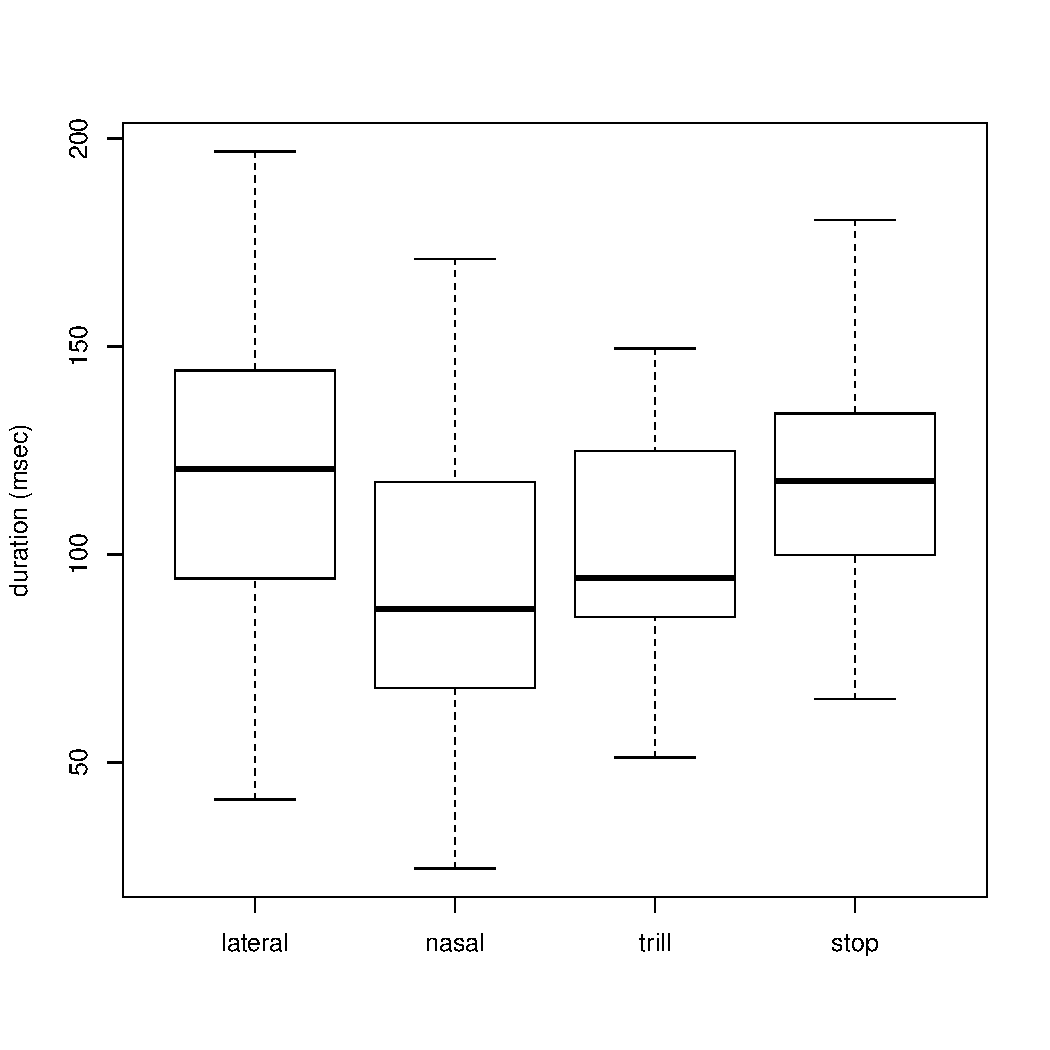
\includegraphics[width=\textwidth]{img/gs-box-1} 

\end{knitrout}
\caption{Duration (in msec) of the glottal spread gesture in sonorants and stops.}
\label{f:spread-box}
\end{figure}

\section{Duration of sonorant consonants}



%\begin{figure}
%\centering
%<<mann-dur-box>>=
%boxplot(dur_mann ~ asp + manner, data = results_son)
%@
%\caption{Duration of sonorant consonants (in msec).}
%\label{f:dur_man}
%\end{figure}

\ctable[caption = Mean duration and standard deviation of sonorants (msec).,
label = t:sonduration
]{lllll}{}{
& \multicolumn{2}{c}{voiced} & \multicolumn{2}{c}{voiceless} \ML
& mean & sd & mean & sd \ML
nasals & 120.41 & 27.19 & 135.09 & 32.03 \NN
laterals & 106.13 & 26.78 & 142.78 & 31.24 \NN
trills & 75.86 & 21 & 125.57 & 32.54 \LL
}

The duration of voiced sonorant consonants was significantly different from the duration of voiceless sonorants.
As a trend, the voiceless sonorants are longer in duration than the voiced ones.
This is not surprising, since voiceless sonorants are less salient from a perceptual point of view.
\citet{silverman1997} argues that, in terms of perceptual optimality, the phasing of non modal voicing in sonorants should involve what he calls truncation of the contrastive laryngeal gesture in respect to the oral ones.
This solution involves the sequencing of non-modal phonation before modal phonation.
According to this principle, an optimal phasing of voicelessness in nasals is achieved when the glottal abduction gesture is terminated before the oral occlusion is released.
In the case the abduction gesture is sequenced before modal voicing, the first portion of the nasal consonant is voiceless (with nareal friction noise), then modal voicing follows.
If, on the contrary, glottal spread follows modal voicing, the last portion of the nasal is characterised by breathy voice.

With laterals, instead, there are two possible optimal phasings of glottal spreading.
In the first type, the abduction of the vocal folds and the lateral tongue gesture are simultaneous.
A voiceless lateral produced in this way normally results in a voiceless lateral fricative more than than an approximant.
In a second type of phasing, the laryngeal abduction is truncated in a similar way as in nasals.
\citet{silverman1997} ascribes such difference in the ways nasals and laterals achieve an optimal phasing of non-modal phonations to a combination of two factors: (1) all laterals are phonetically similar and (2) lateral consonants are easily distinguishable from non-laterals.
%TODO maybe more on this?
The first factor explains why laryngeal distinctions in laterals are cross-linguistically rare, while the second accounts for the higher variability of realizations of laterals compared to that of nasals.
Moreover, these results are similar to those in \citet{jessen1998}, \citet{bombien2006} and \citet{silverman2012}.

%TODO why trills have less variance









\chapter{Discussion}
\label{c:discussion}
%TODO say that of course voicing does not stop, what about breathy voicing!

The research hypothesis of this study is based on the idea that the aspiration effect could be the product of the relative timing of the glottal spread gesture in relation to the tongue gestures in the oral cavity.
An early timing of glottal spread would shorten the vowel, while a later timing would lengthen it.
In particular, the hypothesis states that, in Icelandic, vowels followed by aspirated consonants (pre-aspirated geminates and voiceless sonorants) should be shorter than vowels followed by plain consonants.
As shown in the result chapter (\Cref{c:results}), I found a significant difference between the duration of the vowel in words with aspirated consonants and its duration in words with non-aspirated consonants.
This finding seems to support the timing hypothesis.

\section{Geminate stops}
%ADD many figures
%TODO compare with Ladefoged: he says glottal opening is timed the same and its same apmplitude but is it true here?
We have seen that the absolute duration of vowels is smaller when they are followed by a pre-aspirated geminate than when they are followed by a plain geminate.
It is worth noting that the VOR of the two classes is different, as said in .
However, the fact that the vowel is shorter in words with pre-aspirated geminates cannot be attributed to differences in the over-all duration of the interval between the onset of voicing and the release of the stop.
This is because the VOR is \textit{longer} in words with aspiration while the absolute duration of the vowel is \textit{smaller}.
Other things being equal, we would expect the interval between voice onset and the onset of glottal abduction in words with pre-aspiration to take the same ratio of the VOR as the voiced interval in words with plain geminates.
Instead, laryngeal spreading starts quite early in the word, while voicing is still active even after glottal spread is initiated.

It can be then argued that the relative earlier timing of glottal abduction reduces the vocalic portion where modal voicing is maintained.
This kind of alignment results in a shorter vowel, if we consider the vowel to be the modal voiced interval of the vocalic gesture.
Moreover, when breathy voicing (which is voicing with concomitant abducted vocal folds) is visible from the spectrogram, it should be assumed that the spreading gesture has already reached the critical point in which the abduction is enough to produce breathiness.
This would imply that the gestured might have started even earlier, strengthening the central idea proposed in this research.

However, the hypothesis rested on the idea that voicing would cease earlier in vowels followed by pre-aspirated stops, resulting in a shortened vowel.
What I found, instead, points to a longer voicing portion in words with pre-aspirated stops.
The duration of voicing is, in fact, greater in words with pre-aspirated stops than in words with plain geminates.
This is not surprising, since glottal spread is not incompatible with voicing and could actually allow voicing to be maintained longer.
A plain geminate is produced by keeping the closure for a longer time and voicing during closure is more difficult to maintain.
Thus it is natural to expect that, other things being equal, voicing duration would be greater if glottal spread is involved.
This fact does not fit well with the idea that voicing should cease earlier due to glottal spread.
Even if the physiological explanation seems not to hold, the relative timing on itself can be provisionally considered to be right.

\begin{figure}
\centering
\begin{knitrout}
\definecolor{shadecolor}{rgb}{0.969, 0.969, 0.969}\color{fgcolor}
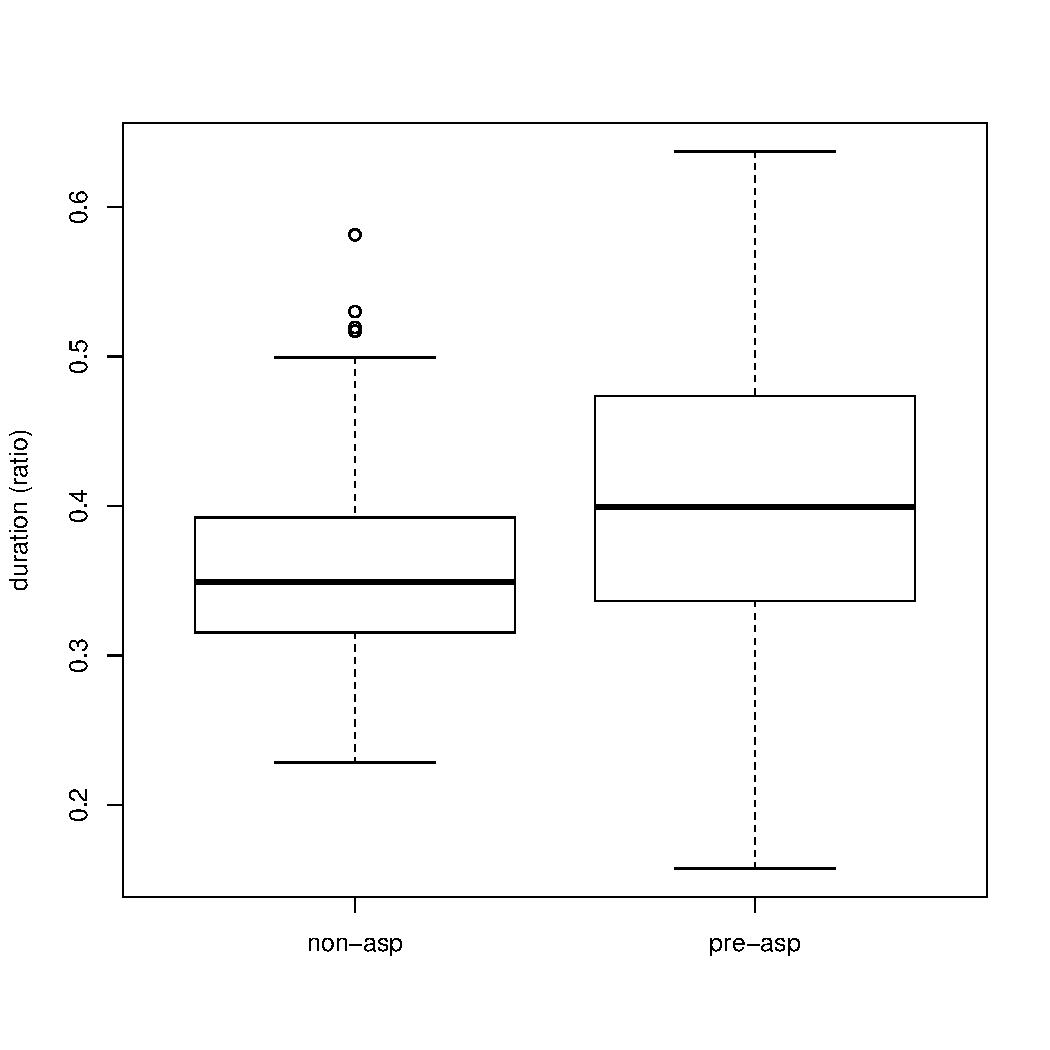
\includegraphics[width=0.8\textwidth]{img/voic-stop-1} 

\end{knitrout}
\caption{Ratio duration of the voicing interval depending on presence or absence of glottal spread.}
\label{f:voicdur}
\end{figure}

Contrary to what stated in \Cref{s:hypothesis}, glottal abduction does not prevent voicing.
On the contrary, longer voicing can be found in words with glottal spread.
A possible explanation of this phenomenon is that the absence of a closure at the VC transition allows for voicing to continue.
In words without glottal spread, the closure of the plain geminate---which is produced immediately after the vowel---quickly produces an increase in oral pressure, until the point is reached when voicing can no longer be sustained.
At the same time, the variance of voicing in the two classes is not the same, and voicing in the aspirated condition has greater variance.
In some aspirated tokens, the duration of voicing is as short---or in a few cases even shorter---than the duration in non-aspirated tokens.

\citet[70--71]{ladefoged1996} state that the glottal width in Icelandic pre-aspirated stops is wider than in non-aspirated stops, but they argue that the timing of glottal spread is the same.
Glottal spread, according to their description, starts at the beginning of the geminate and ends at its release, independently of the presence of pre-aspiration. 
This remark does not fit with the results found in this study.
Although I could not measure glottal width in a direct way, if the description given in \citet{ladefoged1996} is correct, glottal width in non-aspirated geminates can be inferred from the duration of the interval between the offset of voicing of the preceding vowel and the release of the geminate.
Since normalisation was done with the VOR as a base, the portion of VOR subtracted by the modal vocalic portion would correspond to the geminate
Thus, if the ratio duration of glottal spread which should correspond to the duration of the geminate were to be the same both in pre-aspirated and plain stops, the ratio duration of the vowel should have been the same as well.
However, I found that the ratio duration of the vowel was shorter if followed by a pre-aspirated stop.

\section{Sonorants}
%TODO cite previous studies about the duration

The class of sonorant consonants (nasals, laterals and rhotics) seem to pattern together for what concerns durational properties.
As discussed above, all sonorants showed to produce a difference in the ratio duration of voicing depending on whether they were aspirated or not.
Differently from geminate stops, the VOR in words containing sonorant consonants was constant in both the aspirated and non-aspirated classes, except in disyllabic words containing laterals.
The duration of the stop closure after the sonorant was the same in both aspirated and non-aspirated conditions, except with laterals and rhotics in disyllabic words.
The stop consonants in words with /NC/ and /N̥C/ clusters had identical closure durations, so the difference in vowel duration cannot be attributed to closure properties.
The presence vs. the absence of aspiration did not affect the duration of stop closure.

On the contrary, the ratio duration of sonorant consonants (nasal, lateral and rhotic) varied between the aspirated and non-aspirated conditions.
The aspirated sonorants are longer than the non-aspirated ones.
This characteristic can be attributed to perceptual factors.
An aspirated sonorant carries less cues for manner and place of articulation, given that most of it is produced with voiceless noise.
One possible mechanism to enhance manner and place cues and ensure that they are salient enough to be audible is to lengthen the total duration of the sonorant consonant.
This solution would allow more time for sustaining enough modal voicing---which carries better cues than voiceless noise---during the first portion of the sonorant.

In the case of sonorants, it is reasonable to say that the possible cause of shorter vowels in words with aspirated sonorants is the longer duration of the former.
While with stops the VOR is longer with pre-aspirated geminates, with sonorants its duration is the same with aspirated and non-aspirated consonants.
If the speaker intention is to maintain the same VOR while warranting a longer duration of the sonorant, this can be done at detriment of the vowel.
The vowel preceding the aspirated sonorant is thus compressed and it becomes relatively shorter than a vowel followed by a voiced sonorant.
The timing hypothesis presented in this study, thus, seems not to be straightforwardly compatible with the data found in words containing sonorants, even if the effects predicted by it were found.

\section{Linguistic aspects}
This study implicitly assumed that the ultimate origin of the aspiration effect is to be sought in physiological and aerodynamic constraints.
Such constraints could be related to the ways the timing of laryngeal spread is phased in relation to other gestures, as hinted by the results of this research.
However, we cannot exclude the possibility that the speaker is actively varying articulatory gestures either to reduce articulatory effort, to enhance contrast, or both.
\citet[423]{kingston1994} point out that ``speakers and listeners employ extensive and subtle phonetic knowledge.''

In classical models of phonological competence, the articulatory output of the speech stream can be predicted on phonetic grounds from the form of the phonological representation.
This kind of conceptualisation gives the phonetic constraints predictive power.
Knowing which phonological representation underlies a linguistic unit allows us to anticipate the phonetic realisation of that unit. 
\citeauthor{kingston1994}, however, argue that the phonetic constraints normally called for in the literature as the cause of most phonological behaviours do not have predictive power, but rather they limit the possible phonetic outcomes of a phonological abstract unit.
This approach leaves space for the idea that speakers can operate an implicit control over their productions.
The authors call ``phonetic knowledge'' the knowledge underlying such ability.

There are two classes of phonetic knowledge.
The speaker-oriented knowledge deals with the possibilities speakers have to minimise the articulatory effort necessary to produce a particular sequence of gestures (and sounds).
The other type of knowledge, the listener-oriented knowledge, is instead related to the ways speakers can maximise the distinctive cues of contrastive sounds.
Such two kinds of phonetic knowledge work together to create an optimal solution between minimum articulatory effort and maximum contrast.
Borrowing a term from linguistic typology, they can be though of as ``competing motivation'' which shape the phonological systems of the languages of the world.
%TODO citation of competing motivations

We have seen that pre-aspirated stops in Icelandic are preceded by shorter vowels, if we consider the vowel to be the modally voiced open gesture preceding the aspiration.
The magnitude of the difference in duration between vowels followed by pre-aspirated or plain consonants was around 30--40 milliseconds, enough for the auditory system to perceive it.
It is reasonable, thus, to assume that such difference is deliberately used by Icelandic speakers to enhance the contrast between words containing a plain geminate and words with a pre-aspirated geminate.
Even if the original cause of the aspiration effect caused by stops in present day Icelandic could have been related to the phasing of the laryngeal spreading gesture, the synchronic situation we can observe now could instead well be the product of the controlled use of such differences on the part of the speaker.

In the case of sonorants, even if the same shortening effect is seen in vowels followed by aspirated nasals, we cannot claim that the effect is caused by how laryngeal gestures are timed, as explained above.
Instead, the aspiration effect could be attributed here to the fact that voiceless sonorants are generally longer than voiced sonorants so as to enhance cuing.
To maximise even more the difference between voiced and voiceless sonorants, speakers could decrease the duration of the vowel to magnify the longer duration of the sonorant.


%\section{Individual differences}


\section{Diachrony and aspiration effects}
In the previous section I argued that the origin of the effect could be ascribed to timing of laryngeal but that does not mean that synchronically is the case.

%\citet{blevins2013} reports that usually voiceless sonorants develop from clusters including a sonorant and a voiceless consonant (in particular the fricatives /h/ and /s/, see \citealt{palmer1999voiceless} for Kokota and \citealt{Ratliff2001Voiceless} for Hmong-Mien). Other possible origins are word- and phrase-final devoicing and fricatives weakening to voiceless liquids or approximants.

\section{Limitations and challenges}
% participants: diffucult to find in york so the number is not sufficient; age range is quite wide, abroad
% material: difficult to find minimal pairs; there is a contrast but the contrast is not so contrasty
% procedure: they must familiarise with the words first; difficult to control for tempo; differences in compression; different recording equipment and conditions
% annotation: difficulties of finding glottal spread, frame sentence
% articulatory and perceptual study instead
% boundary study, maybe continuos data is better
%TODO limitation of calculating glottal spread

Some of the limitations of this study concern the participants recruited for the reading task.
The first difficulty was finding a sensible number of Icelandic speakers in York.
Due to limitations of time and resources, I could not recruit people from outside York.
This significantly restrained the number of speakers and increased the possibilities that idiosyncrasies could creep into the data.
Moreover, the age range of the participants was quite large (24-66 years old).
The average, though, was biased towards the younger age: 4 out of 6 were within the 24-27 range.
This made conducting age related analyses impossible.
The same argument can be done for sex: 4 out of 6 speakers were female.
There was heterogeneity also in the foreign languages they were confident with.
While Danish was quite common among the youngest speakers, two of them spoke a third language as well (German and Spanish).

Another potential issue with the participants is that all of them, except one, lived in the UK for more than 6 months.
It is reasonable to assume that this had a significant impact on their productions of Icelandic.
Even if the informants allegedly spoke Icelandic on a regular basis, with their family, friends and colleagues, the chances that English influenced Icelandic (and---although not of a concern for the present study---vice versa) are quite high.
The research conducted by \citet{sancier1997} studied how strong the influence was from one language to the other in a Brazilian Portuguese and English bilingual speaker who frequently travelled between Brazil and the United States of America.
The study showed that the speaker produced a shorter voice onset time in both Portuguese and English after spending more than 6 months in Brazil than when she was in the United States.
Thus, it is worth stressing that the results presented here should be taken with a cautionary note.

A further challenge was finding words that would satisfy all of the parameters.
The choice to use real words came at the cost of making the experiment design less balanced.
As mentioned in \Cref{s:materials}, building the word list and controlling for all the criteria while avoiding nonce-words was impossible.
Such gaps in the lexicon of Icelandic show that the functional load of the aspiration contrast is somewhat constrained.
Even if from a more restricted contextual point of view, aspiration contrasts can be found everywhere in the lexicon, true minimal pairs were harder to find.
%TODO add holes and humps paper!

Some design and technical problems arose in the task procedure.
Since the participants did not have the chance to familiarise themselves with the words before starting the task, a few speakers read the first token of some words with uncertainty.
In some cases, they said the wrong word altogether.
One of the speakers (JR) did not recognise most of the inflected words which were not in the standard citation form and decided to read them as if they were English words.
Of course, I had to exclude all of these tokens from the analysis.
This could have been avoided, even if at the cost of less naturalistic data, by letting the speakers read the words beforehand.

A recurrent problem with studies of phonetic duration is that speech tempo is not stable and it is difficult to control.
Using ratio durations can overcome some of the shortcomings of varying tempo.
However, the compressibility of phonetic material is not homogeneous between classes of sounds and contexts.
%TODO add citation

The sound equipment and the recording conditions varied between subjects.
Although the quality of the audio was comparable across recordings, I expect to be minor differences in the way echoes and background noises affected them.
This might have perturbed some speech stretches, in principle rendering visual annotation less reliable.
However, as described in \Cref{s:annotation}, the criteria used during annotation have been devised so as to be consistently applicable.
Such solution substantially reduced possible errors due to the presence of echoes and noises.

Even so, the annotation scheme presented some challenges.
In particular, the visual inspection of the spectrogram was, at times, not unequivocal.
Especially with glottal abduction, I have encountered some difficult tokens where the shape of the waveform did not clearly indicate the onset of breathiness.
In such cases I had to rely only on a change in the look of the spectrogram.
In particular, the results concerning the duration of the spreading gestures are to be taken with caution.
In fact, it is possible that the difference found between stops and sonorants (where the duration of glottal abduction was higher in the former) could be due to the way the measurement was taken.
With sonorants, identifying the beginning of glottal spread by inspecting the waveform or the spectrogram is not straightforward.
Relying on the voiceless portion of the sonorant could potentially leave out the initial part of the spreading gesture.
If one includes such hypothetical part to the duration of spreading, we can expect that the total duration would not be much different in sonorants and stops.

A second aspect of the annotation procedure that presented some difficulties was marking the left and right word boundaries.
Since the frame sentence was kept the same in every trial, words starting and/or ending in a vowel posed problems in identifying the word boundaries.
In such cases, it would not be safe to say that the word duration measurements are unequivocal and reliable.
However, using the VOR instead of the word duration as the base for normalisation guaranteed that errors in the marking of word boundaries would not affect normalisation.

\section{Further studies}

Some of the limitations presented in the previous sections could be overcome with articulatory data.
Laryngeal measures can be taken using photoglottography or a laryngograph.
While the first tool is invasive, the second is not and its portability make its use simple and ideal even in fieldwork conditions.
A laryngograph measures the impedance of the electricity running through the neck.
The amplitude of the impedance is known to be correlated with glottal abduction.
This kind of data would give a better picture of the actions of the glottis and it would allow to retrieve the start of glottal spread with better accuracy.
An ultrasound scanner would provide an account of the gestures of the tongue.
Knowing about tongue movements could make it easier to test for hypothesis that rely on articulatory factors, such as those of ... and ...

Combined with electropalatography, ultrasound scanning can also improve the accuracy of closure detection.
As mentioned above, at times closure is not clearly visible from the spectrogram, especially in cases when voicing is maintained after it.
Tracking the movements of the tongue through ultrasound and palatography can improve the temporal detection of the oral occlusion.
Finally, measuring the oral and the nasal airflows could allow better measurements related to nasals.
The boundary of nasal consonants are normally difficult to discern on the spectrogram.
Voiceless nasals are even more difficult to see, since the friction created at the nostrils is usually very low in amplitude.
Being able to detect nasal airflow allows to clearly define at which time point the velar port has been opened and when it has been closed during speech.

%TODO say about intraoral pressure? for what i dont remember? maybe for saying if voicing is terminated before?















%\chapter{Conclusion}





\appendix

%<<getmeasure, child='rnw/getmeasure.Rnw'>>=
%@





\bibliographystyle{york-harvard}
\bibliography{linguistics}

\end{document}
